
\documentclass[ss]{imsart}

\RequirePackage[OT1]{fontenc}
\RequirePackage{amsthm,amsmath}
\RequirePackage[numbers,sort&compress]{natbib}
\RequirePackage[colorlinks,citecolor=blue,urlcolor=blue]{hyperref}
\usepackage{graphicx}
\usepackage{enumitem}

% settings
\pubyear{2020}
\volume{0}
\issue{0}
\firstpage{1}
\lastpage{8}
% \arxiv{2010.00000}


\startlocaldefs
%\numberwithin{equation}{section}
%\theoremstyle{plain}
%\newtheorem{thm}{Theorem}[section]


%%%%%%%%%%%%%%%%%%%%%%%%%%%%%%
%%%%%%%%%%%%%%%%%%%%%%%%%%%%%%
%%%% This block calls a bunch of useful LaTeX packages
%%%%
%%%%%%%%%%%%%%%%%%%%%%%%%%%%%%
%%%%%%%%%%%%%%%%%%%%%%%%%%%%%%

%\usepackage{algorithm}
\usepackage{amsfonts}
%%\usepackage{amsmath}
%%\usepackage{amsthm}
%%\usepackage{authblk}
%%\usepackage{bibentry}
\usepackage{color}
%\usepackage{epsfig}
%\usepackage{framed}
%\usepackage{graphics}
%%\usepackage{graphicx}
%%\usepackage{hyperref}
%\usepackage{lmodern}
%\usepackage{mathtools}
%\usepackage{pdflscape}
%\usepackage{pdfpages}
%\usepackage{relsize}
%\usepackage{rotating}
%\usepackage{scalerel}
%\usepackage{setspace}
%\usepackage{soul}
%\usepackage{slantsc}
%\usepackage{stackengine}
%\usepackage{subfigure}
%\usepackage{subfiles}
%\usepackage{titlesec}
%%\usepackage{tikz}
%%\usepackage[textsize=footnotesize]{todonotes}   %adding notes on margins
%\usepackage{url}
%\usepackage{verbatim}
%\usepackage{wrapfig}



%\usepackage{natbib}
%%%%%%%%%%%%%%%%%%%%%%%%%%%%%%
%%%%%%%%%%%%%%%%%%%%%%%%%%%%%%
%%%%%%%%%%%%%%%%%%%%%%%%%%%%%%
%%%%%%%%%%%%%%%%%%%%%%%%%%%%%%



%%%%%%%%%%%%%%%%%%%%%%%%%%%%%
%%%%%%%%%%%%%%%%%%%%%%%%%%%%%
%%% This block below is for displaying line numbers properly
%%%
%%%%%%%%%%%%%%%%%%%%%%%%%%%%%
%%%%%%%%%%%%%%%%%%%%%%%%%%%%%
%\usepackage[running, mathlines]{lineno}
%\modulolinenumbers[5]
%\linenumbers
%\newcommand*\patchAmsMathEnvironmentForLineno[1]{%
% \expandafter\let\csname old#1\expandafter\endcsname\csname #1\endcsname
% \expandafter\let\csname oldend#1\expandafter\endcsname\csname end#1\endcsname
% \renewenvironment{#1}%
%    {\linenomath\csname old#1\endcsname}%
%    {\csname oldend#1\endcsname\endlinenomath}}% 
%\newcommand*\patchBothAmsMathEnvironmentsForLineno[1]{%
% \patchAmsMathEnvironmentForLineno{#1}%
% \patchAmsMathEnvironmentForLineno{#1*}}%
%\AtBeginDocument{%
%\patchBothAmsMathEnvironmentsForLineno{equation}%
%\patchBothAmsMathEnvironmentsForLineno{align}%
%\patchBothAmsMathEnvironmentsForLineno{flalign}%
%\patchBothAmsMathEnvironmentsForLineno{alignat}%
%\patchBothAmsMathEnvironmentsForLineno{gather}%
%\patchBothAmsMathEnvironmentsForLineno{multline}%
%}


\newcommand{\BOne}{{\mathbb{1}}}
\newcommand{\BA}{{\mathbb{A}}}
\newcommand{\BB}{{\mathbb{B}}}
\newcommand{\BC}{{\mathbb{C}}}
\newcommand{\BD}{{\mathbb{D}}}
\newcommand{\BE}{{\mathbb{E}}}
\newcommand{\BF}{{\mathbb{F}}}
\newcommand{\BG}{{\mathbb{G}}}
\newcommand{\BH}{{\mathbb{H}}}
\newcommand{\BI}{{\mathbb{I}}}
\newcommand{\BN}{{\mathbb{N}}}
\newcommand{\BP}{{\mathbb{P}}}
\newcommand{\BR}{{\mathbb{R}}}
\newcommand{\BS}{{\mathbb{S}}}
\newcommand{\BT}{{\mathbb{T}}}
\newcommand{\BU}{{\mathbb{U}}}
\newcommand{\BV}{{\mathbb{V}}}
\newcommand{\BW}{{\mathbb{W}}}
\newcommand{\BX}{{\mathbb{X}}}
\newcommand{\BY}{{\mathbb{Y}}}
\newcommand{\BZ}{{\mathbb{Z}}}
\newcommand{\BCOV}{{\mathbb{COV}}}

\newcommand{\cA}{\mathcal{A}}
\newcommand{\cB}{\mathcal{B}}
\newcommand{\cC}{\mathcal{C}}
\newcommand{\cD}{\mathcal{D}}
\newcommand{\cE}{\mathcal{E}}
\newcommand{\cF}{\mathcal{F}}
\newcommand{\cG}{\mathcal{G}}
\newcommand{\cH}{\mathcal{H}}
\newcommand{\cI}{\mathcal{I}}
\newcommand{\cJ}{\mathcal{J}}
\newcommand{\cK}{\mathcal{K}}
\newcommand{\cL}{\mathcal{L}}
\newcommand{\cM}{\mathcal{M}}
\newcommand{\cS}{\mathcal{S}}
\newcommand{\cT}{\mathcal{T}}
\newcommand{\cU}{\mathcal{U}}
\newcommand{\cV}{\mathcal{V}}
\newcommand{\cW}{\mathcal{W}}
\newcommand{\cX}{\mathcal{X}}
\newcommand{\cY}{\mathcal{Y}}
\newcommand{\cZ}{\mathcal{Z}}

\newcommand{\bfalpha}{{\boldsymbol{\alpha}}}
\newcommand{\bfbeta}{{\boldsymbol{\beta}}}
\newcommand{\vecGamma}{{\boldsymbol{\gamma}}}
\newcommand{\bfdelta}{{\boldsymbol{\delta}}}
\newcommand{\bfepsilon}{{\boldsymbol{\epsilon}}}
\newcommand{\bfeta}{{\boldsymbol{\eta}}}
\newcommand{\bflambda}{{\boldsymbol{\lambda}}}
\newcommand{\bfmu}{{\boldsymbol{\mu}}}
\newcommand{\bfnu}{{\boldsymbol{\nu}}}
\newcommand{\bfomega}{{\boldsymbol{\omega}}}
\newcommand{\bfpi}{{\boldsymbol{\pi}}}
\newcommand{\bfpsi}{{\boldsymbol{\psi}}}
\newcommand{\bfsigma}{{\boldsymbol{\sigma}}}
\newcommand{\bftheta}{{\boldsymbol{\theta}}}
\newcommand{\vecXi}{{\boldsymbol{\xi}}}

\newcommand{\bfLambda}{{\boldsymbol{\Lambda}}}
\newcommand{\bfPi}{{\boldsymbol{\Pi}}}
\newcommand{\bfSigma}{{\boldsymbol{\Sigma}}}
\newcommand{\bfTau}{{\boldsymbol{T}}}
\newcommand{\bfTheta}{{\boldsymbol{\Theta}}}
\newcommand{\bfXi}{{\boldsymbol{\Xi}}}

\newcommand{\veca}{{\mathbf {a}}}
\newcommand{\vecb}{{\mathbf {b}}}
\newcommand{\vecc}{{\mathbf {c}}}
\newcommand{\vecd}{{\mathbf {d}}}
\newcommand{\vece}{{\mathbf {e}}}
\newcommand{\vecf}{{\mathbf {f}}}
\newcommand{\vecg}{{\mathbf {g}}}
\newcommand{\vech}{{\mathbf {h}}}
\newcommand{\veci}{{\mathbf {i}}}
\newcommand{\vecj}{{\mathbf {j}}}
\newcommand{\veck}{{\mathbf {k}}}
\newcommand{\vecl}{{\mathbf {l}}}
\newcommand{\vecm}{{\mathbf {m}}}
\newcommand{\vecn}{{\mathbf {n}}}
\newcommand{\veco}{{\mathbf {o}}}
\newcommand{\vecp}{{\mathbf {p}}}
\newcommand{\vecq}{{\mathbf {q}}}
\newcommand{\vecr}{{\mathbf {r}}}
\newcommand{\vecs}{{\mathbf {s}}}
\newcommand{\vect}{{\mathbf {t}}}
\newcommand{\vecu}{{\mathbf {u}}}
\newcommand{\vecv}{{\mathbf {v}}}
\newcommand{\vecw}{{\mathbf {w}}}
\newcommand{\vecx}{{\mathbf {x}}}
\newcommand{\vecy}{{\mathbf {y}}}
\newcommand{\vecz}{{\mathbf {z}}}

\newcommand{\veczero}{{\mathbf {0}}}
\newcommand{\vecone}{{\mathbf {1}}}


\newcommand{\vecA}{{\mathbf {A}}}
\newcommand{\vecB}{{\mathbf {B}}}
\newcommand{\vecC}{{\mathbf {C}}}
\newcommand{\vecD}{{\mathbf {D}}}
\newcommand{\vecE}{{\mathbf {E}}}
\newcommand{\vecF}{{\mathbf {F}}}
\newcommand{\vecG}{{\mathbf {G}}}
\newcommand{\vecH}{{\mathbf {H}}}
\newcommand{\vecP}{{\mathbf {P}}}
\newcommand{\vecQ}{{\mathbf {Q}}}
\newcommand{\vecR}{{\mathbf {R}}}
\newcommand{\vecS}{{\mathbf {S}}}
\newcommand{\vecT}{{\mathbf {T}}}
\newcommand{\vecU}{{\mathbf {U}}}
\newcommand{\vecV}{{\mathbf {V}}}
\newcommand{\vecW}{{\mathbf {W}}}
\newcommand{\vecX}{{\mathbf {X}}}
\newcommand{\vecY}{{\mathbf {Y}}}
\newcommand{\vecZ}{{\mathbf {Z}}}

\newcommand{\vecYb}{{\mathbf {Y}}_{b}}
\newcommand{\vecYOrderi}{{\mathbf {Y}}_{(i)}} 



\newcommand{\vecalpha}{\bfalpha}
\newcommand{\vecbeta}{\bfbeta}
\newcommand{\vecgamma}{\vecGamma}
\newcommand{\vecepsilon}{\bfepsilon}
\newcommand{\veceta}{\bfeta}
\newcommand{\vecmu}{\bfmu}
\newcommand{\vecpi}{\bfpi}
\newcommand{\vectheta}{\bftheta}
\newcommand{\vecxi}{\vecXi}


\newcommand{\vecLambda}{\bfLambda}
\newcommand{\matLambda}{\bfLambda}
\newcommand{\vecPie}{\bfPi}
\newcommand{\matTheta}{\bfTheta}
\newcommand{\matXi}{\vecXi}


\newcommand{\trace}{{\mathrm {tr}}}
\newcommand{\ind}{ \stackrel{ind.}{=} }
\newcommand{\iid}{ \stackrel{i.i.d.}{=} }
\newcommand{\iidold}{ \stackrel{i.i.d.}{\sim} }
\newcommand{\non}{\nonumber}
 \newcommand{\raro}{\rightarrow}
 \newcommand{\Raro}{\Rightarrow}
 \newcommand{\LRaro}{\Leftrightarrow}
\newcommand{\bver}{\begin{verbatim}}
\newcommand{\ever}{\end{verbatim}}

%%%%% Useful for aligned equations
\def\baq#1\eaq{\begin{align}#1\end{align}}
\def\ban#1\ean{\begin{align*}#1\end{align*}}

%%%%% A tool for defining inner products
\def\binner#1\einner{\bigl\langle #1 \bigr\rangle}

\newcommand{\MyBox}{ \raisebox{0.8mm}{\scalebox{0.5}{\fbox{\parbox[t][0.5mm][t]{0.75mm}{}}}}}

\def\bBP #1\eBP{\BP \bigl[ #1 \bigr]}
\def\BeginRedComment#1\EndRedComment{({\color{red}{\bf Comment:} {\it #1}}) }
\def\BeginBlueComment#1\EndBlueComment{({\color{blue}{\bf Comment:} {\it #1}}) }


   \newtheoremstyle{Example}{\topsep}{\topsep}%
     {}%         Body font
     {}%         Indent amount (empty = no indent, \parindent = para indent)
     {\bfseries}% Thm head font
     {:}%        Punctuation after thm head
    {0.9mm}%     Space after thm head (\newline = linebreak)
     {\thmname{#1}\thmnumber{ #2}\thmnote{(\it #3)}}%         Thm head spec
		
%	\AtEndEnvironment{Example}{\null\hfill\qed}%
   \theoremstyle{Example}
   \newtheorem{Example}{Example}[section]
	\AtEndEnvironment{Example}{\null\hfill\qed}%


\endlocaldefs

%%%%%%%%%%%%%%%%%%%%%%%%%%%%%%
%%%%%%%%%%%%%%%%%%%%%%%%%%%%%%
%%%%%%%%%%%%%%%%%%%%%%%%%%%%%%
%%%%%%%%%%%%%%%%%%%%%%%%%%%%%%


%%%%%%% Commands for commenting
%\usepackage{color}
\newcommand{\remove}[1]{ }
%\newcommand{\revised}[1]{{\color{red}{#1}}}
\newcommand{\attention}[1]{{\color{red}{\textbf{[ATTENTION:#1]}}}}
\newcommand{\NeedToChange}[1]{{\color{blue}{\textbf{[NEED to CHANGE:]}\textit{#1}}}}
%\newcommand{\todo}[1]{{\color{blue}{[TO DO: #1]}}}
\newcommand{\mycomment}[1]{{\color{blue}{[#1]}}}
%\newcommand{\addref}{\mycomment{ADD REF}}
%\newcommand{\update}[1]{{\color{green}{#1}}}
%\newcommand{\new}[1]{{\color{blue}{#1}}}
%%%%%%%%%%%%%%%%%%%


%%%%%%%%%%%%%%%%%%%%%%%%%%%%%%
%%%%%%%%%%%%%%%%%%%%%%%%%%%%%%
%%%%%%%%%%%%%%%%%%%%%%%%%%%%%%
%%%%%%%%%%%%%%%%%%%%%%%%%%%%%%
%\voffset=-0.5in
%
%\renewcommand{\baselinestretch}{1.15}




\begin{document}


\begin{frontmatter}

\title{Robust Methods for Principal Component Analysis: A Contemporary Review
% \support{Acknowledge grants here}
}
\runtitle{Robust PCA}

\begin{aug}
\author{\fnms{Subhabrata} \snm{Majumdar}\thanksref{t1}\ead[label=e1]{smajumdar@splunk.com}}
\and
\author{\fnms{Sarah} \snm{Sernaker}\thanksref{t2}\ead[label=e2]{second@somewhere.com}}
\and
% \address{Address of the First and Second authors\\
% usually few lines long\\
% \printead{e1,e2}}
\author{\fnms{Snigdhansu} \snm{Chatterjee}\thanksref{t3}
\ead[label=e3]{chatt019@umn.edu}
\ead[label=u1,url]{http://users.stat.umn.edu/~chatt019/}}

\address{School of Statistics\\
University of Minnesota\\
313 Ford Hall, 224 Church Street S.E., Minneapolis, MN 55455\\
\printead{e1,e2,e3}\\
\printead{u1}}

\thankstext{t1}{Currently at Splunk.}
\thankstext{t2}{Something}
\thankstext{t3}{SC acknowledges partial support for this work from ???}
\runauthor{S. Majumdar et al.}
\end{aug}


\begin{abstract}
We review several proposed techniques for robust principal component analysis (PCA), including projection pursuit PCA, matrix decomposition techniques like principal component pursuit, low-leverage decomposition, robust subspace recovery, PCA on multivariate signs and weighted multivariate signs where the weights may depend on data-depth, and random projection and subsetting approaches. We consider statistical consistency, efficiency and robustness properties, as well as computational complexities of the proposed techniques. We apply these techniques on variants of the Iris data, on examples from the Face Database B, and on the MNIST data. Our analyses suggest that PCA on generalized signs and weighted signs are very strong candidates for robust PCA, while techniques like random subsetting and projections and matrix decomposition ideas need to be studied further. 
\end{abstract}

\begin{keyword}[class=MSC]
\kwd[Primary ]{60K35???}
\kwd{60K35???}
\kwd[; secondary ]{60K35???}
\end{keyword}

\begin{keyword}
\kwd{Principal Component Analysis}
\kwd{robustness}
\kwd{projection pursuit}
\kwd{spatial signs}
\kwd{data depth}
\kwd{principal component pursuit}
\end{keyword}
\tableofcontents
\end{frontmatter}


%\abstract{
%We review several proposed techniques for robust principal component analysis (PCA), including projection pursuit PCA, matrix decomposition techniques like principal component pursuit, low-leverage decomposition, robust subspace recovery, PCA on multivariate signs and weighted multivariate signs where the weights may depend on data-depth, and random projection and subsetting approaches. We consider statistical consistency, efficiency and robustness properties, as well as  computational complexities of the proposed techniques. We apply these techniques on variants of the Iris data, the MNIST data and datasets on images (?). Our analyses suggest that PCA on generalized signs and weighted signs are very strong candidates for robust PCA, while techniques like random subsetting and projections and matrix decomposition ideas need to be studied further. 
%}

\newpage
\section{Introduction}

\textrm{Principal Components Analysis} (PCA often hereafter) was introduced  in 
\cite{ref:JEducationalPsychology33417_Hotelling_PCA} and 
\cite{ref:JEducationalPsychology33498_Hotelling_PCA}, as a tool for studying multivariate data.  However, an earlier iteration of this concept, presented in the context of total least squares (in today's terminology), may be found in \cite{ref:Pearson1901559_PCA}.
\attention{Provide 2-3 additional references and names from wikipedia.}

%; the Wikipedia page on PCA 
%(\url{https://en.wikipedia.org/wiki/Principal_component_analysis}) 
%contains more historical and appellative references. 



We use the notation $\delta_{j k}$ for the Kronecker delta, that is, $\delta_{j k} = 1$ if $j = k$ and zero otherwise. The notation $a^{T}$ denotes the transpose of any finite-dimensional vector or matrix $a$,  $|| a ||$ denotes the Euclidean norm of the vector $a$, and for any two vectors $a$ and $b$ of identical dimension,  $\langle a, b \rangle $ denotes the Euclidean inner product. All vectors are assumed to be column vectors in this paper. For a positive definite matrix $\Sigma \in \BR^{p \times p}$, the spectral decomposition yields $\Sigma = \BP \Lambda \BP^{T}$, where the columns of the orthogonal matrix $\BP$ are the eigenvectors of $\Sigma$ corresponding to the eigenvalues $\lambda_{1} (\Sigma) \geq \lambda_{2} (\Sigma) \geq \ldots \lambda_{p} (\Sigma) > 0$, where$\lambda_{i} (\Sigma)$ denotes the $i$-th diagonal element of $\Lambda$. The notation $\Sigma^{\alpha}$ for $\alpha \in \BR$ is defined as $\Sigma^{\alpha} = \BP \Lambda^{\alpha} \BP^{T}$, where  $\Lambda^{\alpha}$ is the diagonal matrix with $i$-th diagonal element $\lambda_{i}^{\alpha} (\Sigma)$. For a real matrix $A \in \BR^{a \times b}$ of rank $r$, the singular value decomposition obtains the factorization $A = U S V^{T}$ where $U$ and $V$ are orthogonal matrices, and $S$ is a diagonal matrix with exactly $r$ positive diagonal entries $\sigma_{1} (A), \ldots, \sigma_{r} (A)$ that are known as \textit{singular values}. 



Given a dataset  ${\BX} = ( \BX_{1}: \ldots : \BX_{n} )^{T} \in \BR^{n \times p}$, whose rows  $\{ {\BX}_{i} \in \BR^{p}: i =1, \ldots, n \}$ are measurements on $p$ variables,  the first step towards PCA is typically to subtract the column-wise means (sample mean of each variable) 
$\bar{\BX}_{n} = n^{-1} \sum_{i = 1}^{n} \BX_{i} \in \BR^{p}$, to obtain 
$X_{i} = \BX_{i} - \bar{\BX}_{n}, \ i = 1, \ldots, n$, and the centered matrix 
$\vecX = ( {X}_{1}: \ldots : {X}_{n} )^{T} \in \BR^{n \times p}$. Then typically, a collection of unit norm, mutually orthogonal vectors 
$G_{1}, G_{2}, \ldots, G_{k} \in \BR^{p}$ are obtained (thus 
$G_{j}^{T} G_{k} = \delta_{j k}$), such that the sample variances
\baq 
V_{j} = (n - 1)^{-1} \sum_{i = 1}^{n} \Bigl( 
G_{j}^{T} {X}_{i} - n^{-1} \sum_{i = 1}^{n} G_{j}^{T} {X}_{i}
\Bigr)^{2}
= (n - 1)^{-1} \sum_{i = 1}^{n} \Bigl( 
G_{j}^{T} {X}_{i} \Bigr)^{2}
\label{eq:PCA1}
\eaq 
form a non-increasing sequence, thus $V_{1} \geq V_{2} \geq  \ldots \geq V_{k}$. 
Thus, $G_{1}$ is obtained  by optimizing $\arg \max_{| v | = 1} \sum_{i = 1}^{n} | \langle {X}_{i}, v \rangle |^{2}$, $G_{2}$ obtained  by optimizing $\arg \max_{| v | = 1, \langle v, G_{1} \rangle = 0} \sum_{i = 1}^{n} | \langle {X}_{i}, v \rangle |^{2}$, and so on.  
The vector $H_{j} = {\vecX} G_{j} \in \BR^{n}$ is generally referred to as the $j$-th principal component. The mutual orthogonality of $G_{1}, G_{2}, \ldots, G_{k}$ further ensures that $H_{1}, H_{2}, \ldots, H_{k}$ have zero sample covariances between themselves. The above scheme may be implemented up to $k = \min \{ n - 1, p \}$. To simplify notations for the discussion  below, define the matrices $\vecG = (G_{1}: G_{2}: \ldots :G_{k}) \in \BR^{p \times k}$ and $\vecH = (H_{1}: H_{2}: \ldots :H_{k}) \in \BR^{p \times k}$, as  the \textit{sample eigenvectors} and the projection of the centered data on these eigenvectors. The latter is often referred to as  \textrm{principal component scores (or PC scores)}, we will refer to these as \textit{PC-projections} so as not to confuse with the multiple other uses of the term ``score'' in statistics and data sciences. 


It is important to realize that PCA is a \textit{sample-driven} property, that is, $\vecG$ and consequently  the principal components $\vecH$ depend on the observed data $\vecX$. In particular, these are sensitive to the scaling of the different variables, and to aberrant observations in the data. In addition, the distributional properties of $\vecG$ are nontrivial when he number of variables $p$ is large compared to the sample size $n$.

This  review concentrates on the \textit{robustness} studies on PCA. 
% \attention{Add several more lines here on what is being reviewed.}
{\color{red}
While extensive research (and reviews) have been done on this subject before, we focus on relatively new methodological developments, specifically those driven by cutting-edge applications.
}
For convenience of presentation, we consider a part of the well known \textrm{Iris flower data} \cite{fisher1936use} as an illustrative example throughout the paper. This data consists of four measurements (sepal and petal lengths and widths) on each three species of Iris flower, \textit{ Iris Setosa, Iris Virginica} and \textit{Iris Versicolor}, with fifty independent measurements from each species. For illustrating the usage of different robust PCA techniques, we use the data on sepal lengths and widths for the \textit{Iris setosa} flower, and replace a single with an outlier. Later in Section~\ref{Sec:DataExpt} we consider more substantial data examples that have more observations and variables.



\begin{figure}
\begin{center}
\begin{tabular}{cc}
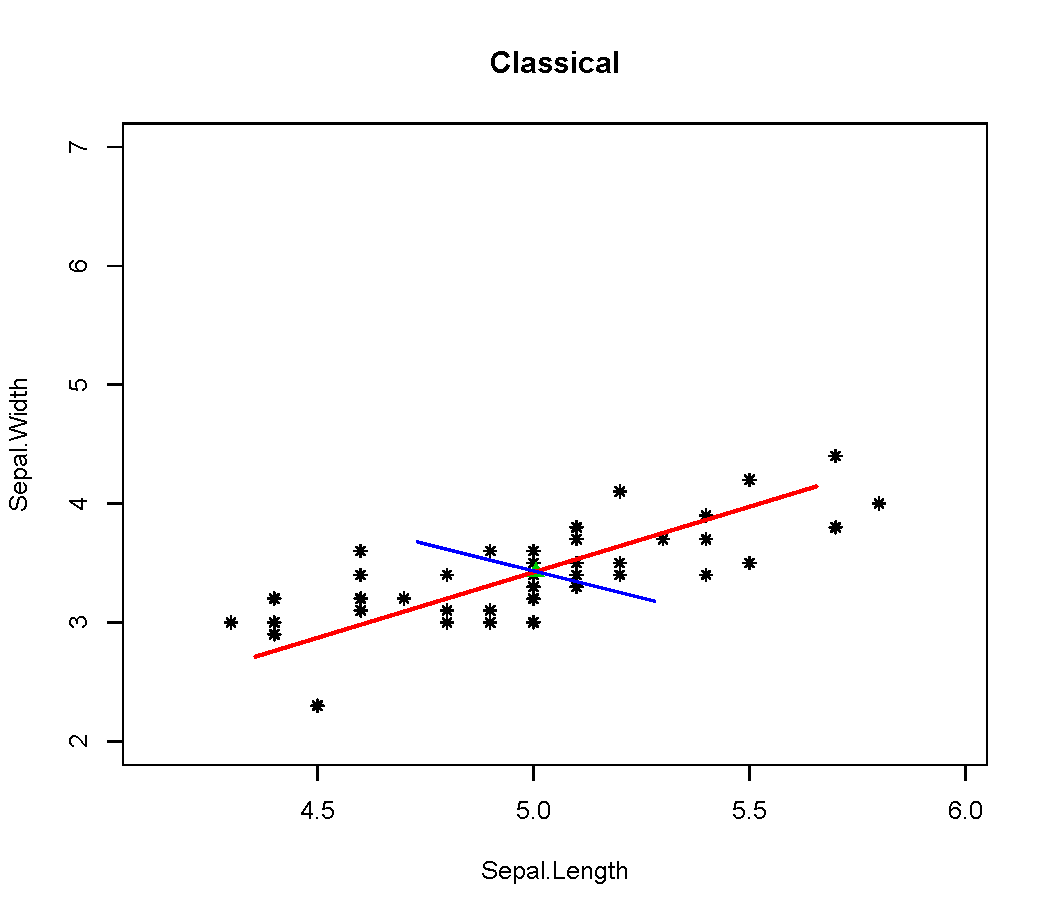
\includegraphics[width=0.49\textwidth]{./RobustPCA_Figures/Iris_Sepal_PCA_Orig} &
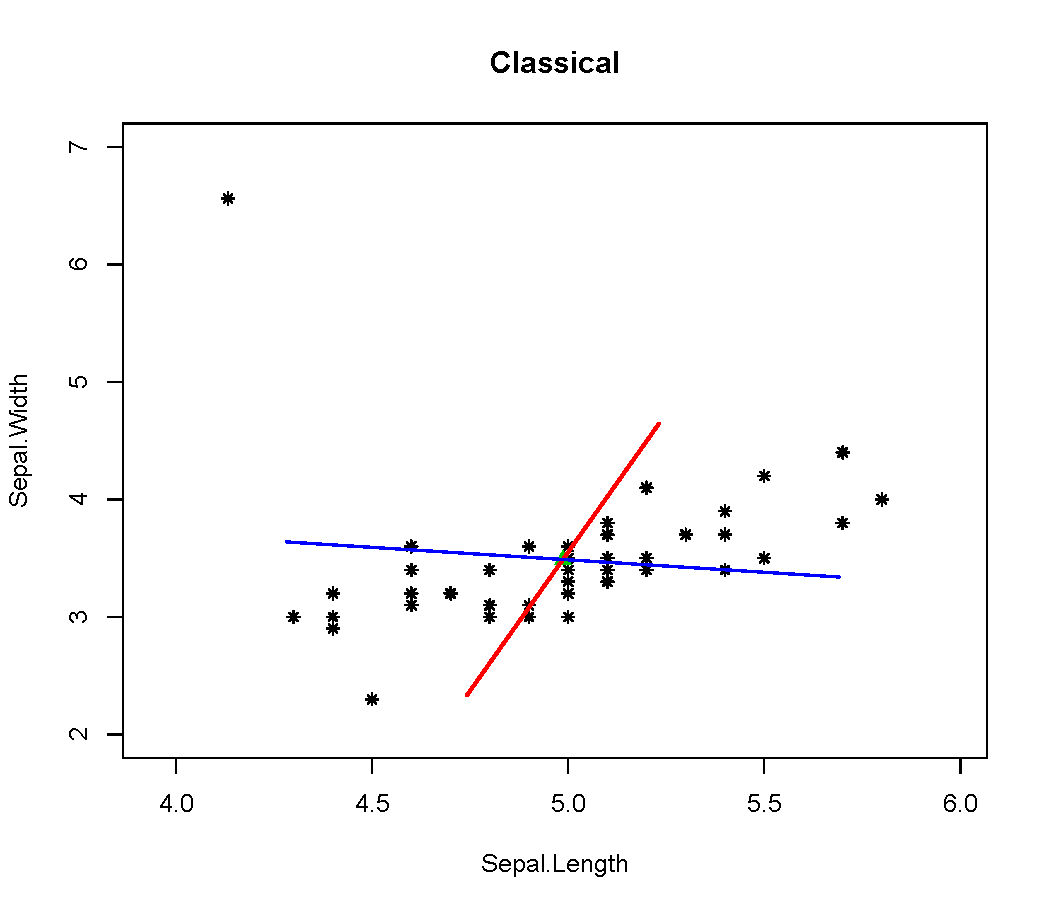
\includegraphics[width=0.49\textwidth]{./RobustPCA_Figures/Iris_Sepal_PCA_Out} 
\end{tabular}
\end{center}
\caption{The sepal length and width of \textit{Iris Setosa}. The left panel shows the original data with the principal components, computed using the classical PCA algorithm. The first principal component is in red, and the second in blue. The right panel is the same data with a single randomly generated outlier, visible in the top left corner, and  its resulting effect on the classical principal components. }
\attention{The caption on the right figure should say "Classical with Outlier"}
\label{Figure:1}
\end{figure}

\begin{Example}
We demonstrate the fragility of classical PCA and the need for robust PCA using Figure~\ref{Figure:1}. The left panel shows the sepal length and width data of \textit{Iris Setosa} from the Iris data \cite{fisher1936use}, and two corresponding principal components derived from classical PCA. The first principal component is depicted in red, and the second in blue. In the right panel, one data point is replaced with a random outlier, visible near the top left corner of the figure, and the classical PCA is reapplied. Notice how greatly both principal components have become distorted.  
\end{Example}


\paragraph{The model.}
While PCA is a sample-driven technique, it is worthwhile to reflect on the model at a population level, since that sets the context under which robustness may be desired. Throughout this paper, we assume that $p$ is fixed, and that the $p$-dimensional observations are independent and identically distributed (iid often hereafter). We assume that all the observations $\BX_{1}, \ldots, \BX_{n}$ share a common location $\mu \in \BR^{p}$ and a common positive definite scatter matrix $\Sigma \in \BR^{p \times p}$. A generative model can be $\BX_{i}$'s are iid $N_{p} (\mu, \Sigma)$, the $p$-dimensional Gaussian  distribution with mean $\mu \in \BR^{p}$ and positive definite variance $\Sigma$. Another generative model is where  $\Sigma^{-1/2} (\BX_{i} - \mu)$ are iid from a $p$-dimensional standard $t$-distribution with $k > 2$ degrees of freedom. 

PCA is routinely used on data with more complex patterns and not just on iid data, for example in spatio-temporally dependent data, but the above model suffices for the present review. \attention{This sentence belongs to the conclusion.}


%\attention{Done up to here.}

We assume that a suitable location estimator $\hat{\mu} \in \BR^{p}$ is used to obtain the centered matrix $\vecX = ( {X}_{1}: \ldots : {X}_{n} )^{T} \in \BR^{n \times p}$, comprised of the vectors $X_{i} = \BX_{i} - \hat{\mu}$. The choice of  a  $\hat{\mu} $   is important: using the non-robust sample mean $\bar{\BX}_{n} = n^{-1} \sum_{i = 1}^{n} \BX_{i} \in \BR^{p}$ may deeply compromise the subsequent PCA. Using coordinate-wise median (or any other multivariate median) requires additional assumptions on the distribution.  

\paragraph{Departures from the model.}
We may allow different kinds of departures from the above model. First, we may allow isolated aberrant observations in any of the $p$ elements of any of the $n$ observations. Second, a $p$-dimensional random vector from a distribution different from that of $\BX_{1}$ may be added to or may be used to replace an entire actual data-point. This rogue contaminant random variable may be anywhere on the support of $\BX_{1}$ or in $\BR^{p}$, e. g. a potential \textit{outlier}, or it may be supported on a lower dimensional manifold in $\BR^{p}$, e. g. an \textit{inlier}. A typical data analysis problem may involve any combination of aberrant observations in one or more coordinates, entire observations as outliers, or entire observations as inliers. 


\paragraph{Desirable properties of robust PCA methods.}
The domains of applications of PCA methods are vast, including social and natural science disciplines, numerous engineering disciplines, as well as modern applications involving machine learning, computer vision and so on \cite{AlkandariAljaber15,AlexanderBook,WilksBook,BerryCastellanos}. %\attention{Need citations here}
Consequently, we have seen many conceptual proposals of robust PCA methodology over the last several decades, often accompanied by different theoretically established robustness properties or practical demonstrations of robustness. In modern times, computational aspects and efficiency of the algorithm also need to be considered. Also, several proposed algorithms are based on deterministic frameworks and did not consider the stochastic aspects of data
{\color{red}
---such as matrix completion approaches \cite{CandesTao10,Vaswani}}. Consequently, the compatibility of robust PCA algorithms to noise and stochasticity in data also needs to be considered. %\attention{The sentences above need citations, or some statement that we will cite these later.}

We propose the following as a list of desirable properties for a robust PCA method:
%
\begin{enumerate}[label=\alph*),leftmargin=*]
\setlength\itemsep{0em}
    \item It should provide reasonable and provable robustness guarantees against the different kinds of data aberrations listed above.
    \item It should lead to reasonable parameter estimates and other statistics with provable efficiency guarantees.
    \item It should be computable in realistic time, with computational complexity guarantees.
    \item It should be robust against the presence of noise and stochasticity in the data.
    \item The assumed population distribution---or deterministic structure---should be clearly stated and transparent.
    \item It should be amenable to detailed theoretical analysis to ensure uncertainty quantification and statistical inference,  and for use in a complex data analysis exercise that involved several procedures other than PCA.
    \item The outputs should be interpretable along the lines of traditional PCA.
    \item There should be accessible code implementing these algorithms in standard statistical softwares.
\end{enumerate}

The properties one may want for a robust PCA algorithm naturally depend on the context and the priorities of the researcher. The above generic list has been framed keeping in mind that in many modern applications, a robust PCA procedure may be part of a `blackbox' algorithm that is repeatedly used by an analyst on different kinds of large and intractable datasets, where it is infeasible to tweak parts of the algorithm of monitor each data analysis step and speed is of essence. Yet when necessary,  the scientist may prise open the blackbox to satisfy herself that the component procedures follow robustness and efficiency standards, or to develop better algorithms. An example of the above may be a software used by banks and financial institutions to machine-read personal checks with handwritten entries, or a software that converts comments by medical personnel into specific keywords on a person's electronic healthcare record. 

\paragraph{Structure of review.}
We group algorithms for robust PCA into four groups, based on the techniques used and the underlying assumptions. These are ($i$) projection pursuit PCA methods that have appeared in statstics literature typically around two decades back, reviewed in Section~\ref{Sec:PP_PCA} below; ($ii$) matrix decomposition methods that have overwhelmingly appeared in the machine learning and applied mathematics literature, reviewed in Section~\ref{Sec:MatDec_PCA}; ($iii$) PCA on multivariate signs with or without weights, which have been reported to perform well by multiple authors, reviewed in Section~\ref{Sec:Sign_PCA}; and ($iv$) PCA methods on random subsets and random projections of the data, which leverage some of the lessons learned for obtaining high-dimensional PCAs, reviewed in Section~\ref{Sec:RanProj_PCA}. We also collect some additional approaches that do not fit the above groups well in Section~\ref{Sec:Misc_PCA}, and report two comparative studies of robust PCA techniques using real data in Section~\ref{Sec:DataExpt}. Concluding remarks are presented in Section~\ref{Sec:Conclusion}. 


%\attention{Done up to here.}


\section{Projection Pursuit PCA}
\label{Sec:PP_PCA}


The sensitivity of the classical PCA arises from using the sample mean for centering and the sample variance as the optimization (maximization) criterion, both of which have zero breakdown value. The projection pursuit approach to PCA proposes using  robust measures of location and scale instead. First proposed in \cite{ref:JASA85759_RPCA}, this method has been thoroughly explored in papers on robust PCA published in the twentieth century and the early part of the twenty-first century. 

A typical example of a projection pursuit PCA is in the use of robust covariance or correlation estimators. For example in   \cite{ref:Biometrika00603_CrouxHaesbroeck_RPCA}, 
authors consider  the data to be iid $N_{p} (\mu, \Sigma)$ with fixed $p$, and 
assume that $\Sigma$ has distinct eigenvalues 
 $\lambda_{1} > \lambda_{2} > \ldots \lambda_{p} > 0$ with eigenvectors 
 $v_{1}, \ldots, v_{p}$. In this framework, they
study three choices for robust location and scatter: 
($a$) the $M$-estimator of \cite{ref:AoS7651_Maronna_Robust}, 
($b$) the $S$-estimator of \cite{rousseeuw2005robust}
%, page 263 
and \cite{ref:AoS871269_Robust}, and ($c$) the one-step reweighted minimum covariance determinant estimator \cite{rousseeuw1985multivariate}. 
They recommend $S$-estimators of $\Sigma$, for which high efficiency as well as robustness properties are obtainable \cite{ref:Test14356_SEstimator, ref:SJS11332_Croux_SEstimator}, but low efficiency in regression is also a possibility \cite{ref:SPL92413_SEstimator}. 

Computations of projection pursuit-based principal components can be challenging. For example, preliminary estimators of location and scale often required in the algorithm need $O (n^{\alpha n})$ computational steps, for some 
$\alpha \in (0, 1)$. Subsequent calculations further increase the computational burden. Also, the use of multi-stage estimation techniques can lead to non-standard asymptotics. 
Developments related to projection pursuit-based PCA approaches may be found in 
\cite{ref:JASA93505_PCA, ref:AISM98471_PCA, ref:SPL99349_PCA, ref:Biometrika03953_Cuietal_RPCA, ref:IJCV03117_RPCA, ref:Technometrics0564_Hubert_RPCA, ref:Technometrics05264_Maronna_RCPA, ref:JMVA05206_RPCA_Croux, ref:CSDA061441_RPCA, croux2007algorithms, ref:IEEETransPAMI081672_RPCA, ref:Technometrics13202_Croux_PCA, ref:Biometrika15573_PCA}.

We experimented with several \texttt{R} packages and program choices for obtaining projection pursuit-based principal components. These include 
the functions \texttt{robpca} and \texttt{rospca} from the library \texttt{rospca},
the functions \texttt{PCAgrid} and \texttt{PCAproj} from the library \texttt{pcaPP},
the function \texttt{GSE} from the library \texttt{GSE}, 
the function \texttt{prcomp.robust} from the library \texttt{mdqc}, 
the function \texttt{SPcaGrid} from the library \texttt{rrcovHD}. If a package did not contain a robust location estimator, we use the coordinatewise median.
%
 \begin{figure}
\begin{center}
\begin{tabular}{ccc}
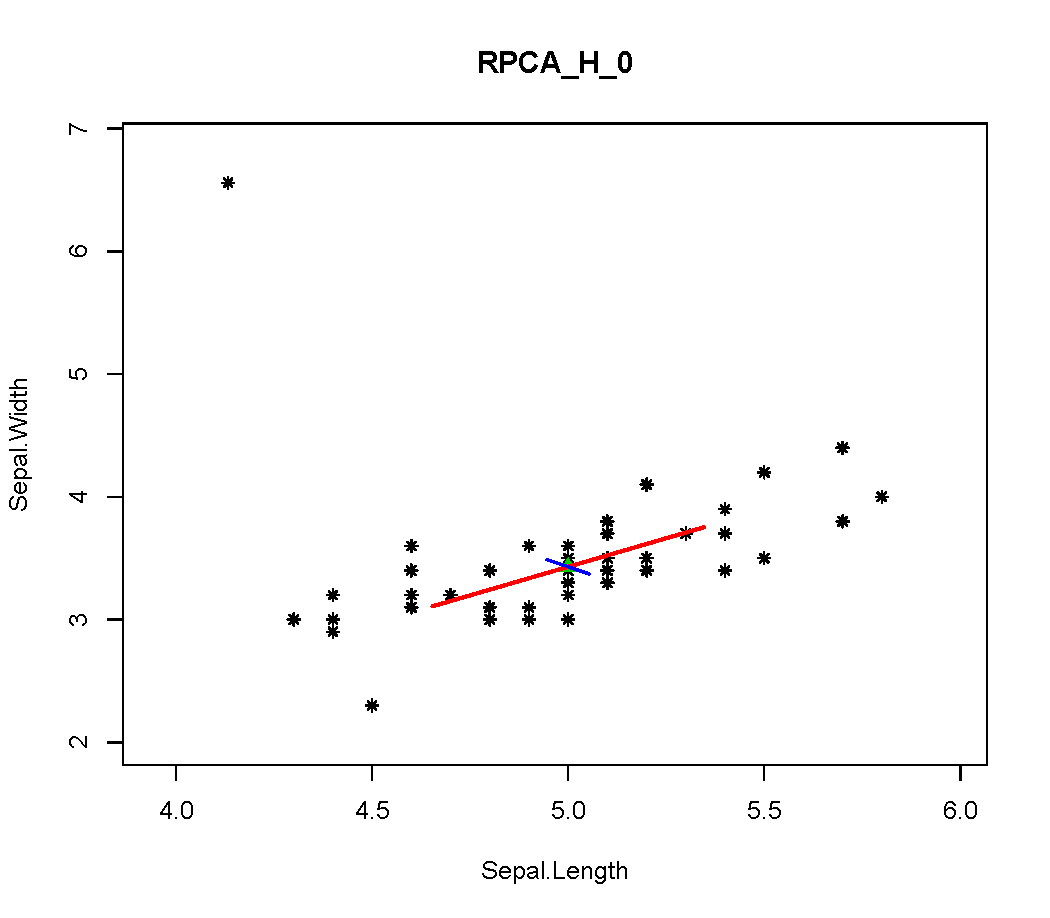
\includegraphics[width=0.3\textwidth]{./RobustPCA_Figures/Iris_Sepal_PCA_Out_H0} &
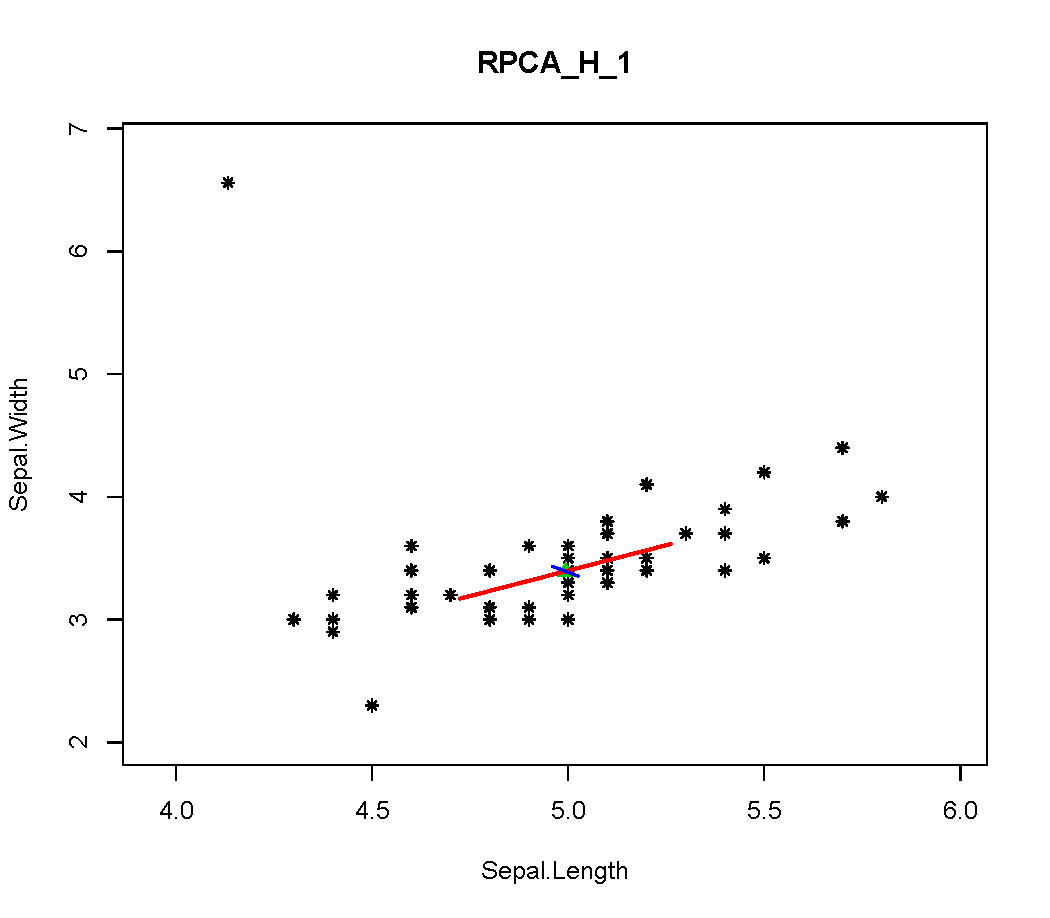
\includegraphics[width=0.3\textwidth]{./RobustPCA_Figures/Iris_Sepal_PCA_Out_H1} &
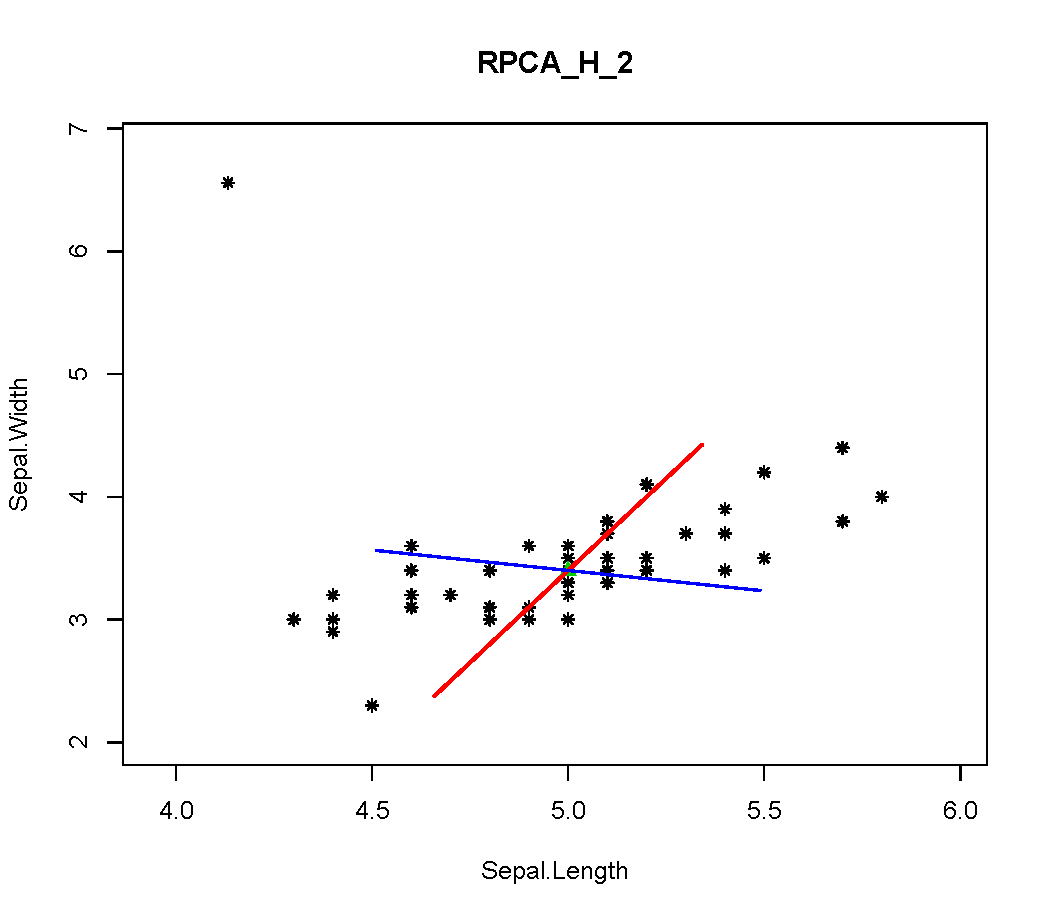
\includegraphics[width=0.3\textwidth]{./RobustPCA_Figures/Iris_Sepal_PCA_Out_H2} \\
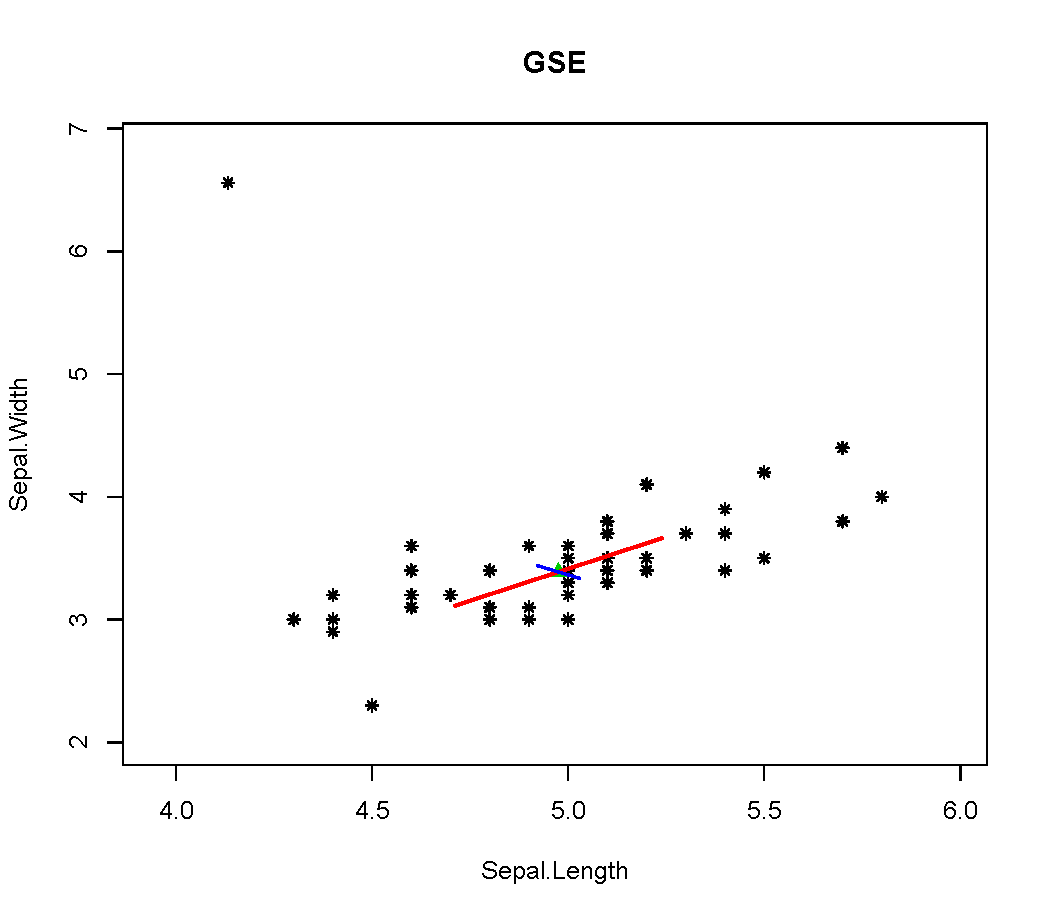
\includegraphics[width=0.3\textwidth]{./RobustPCA_Figures/Iris_Sepal_PCA_Out_GSE} &
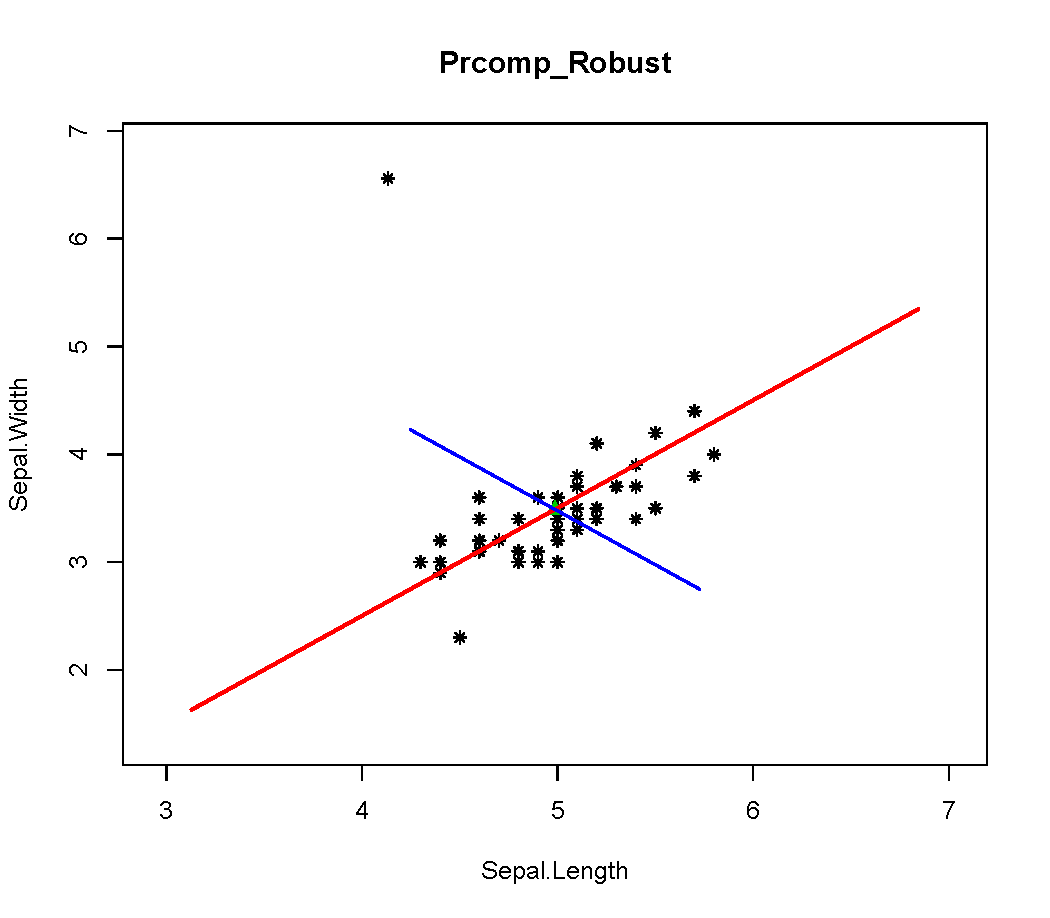
\includegraphics[width=0.3\textwidth]{./RobustPCA_Figures/Iris_Sepal_PCA_Out_PRRobust} &
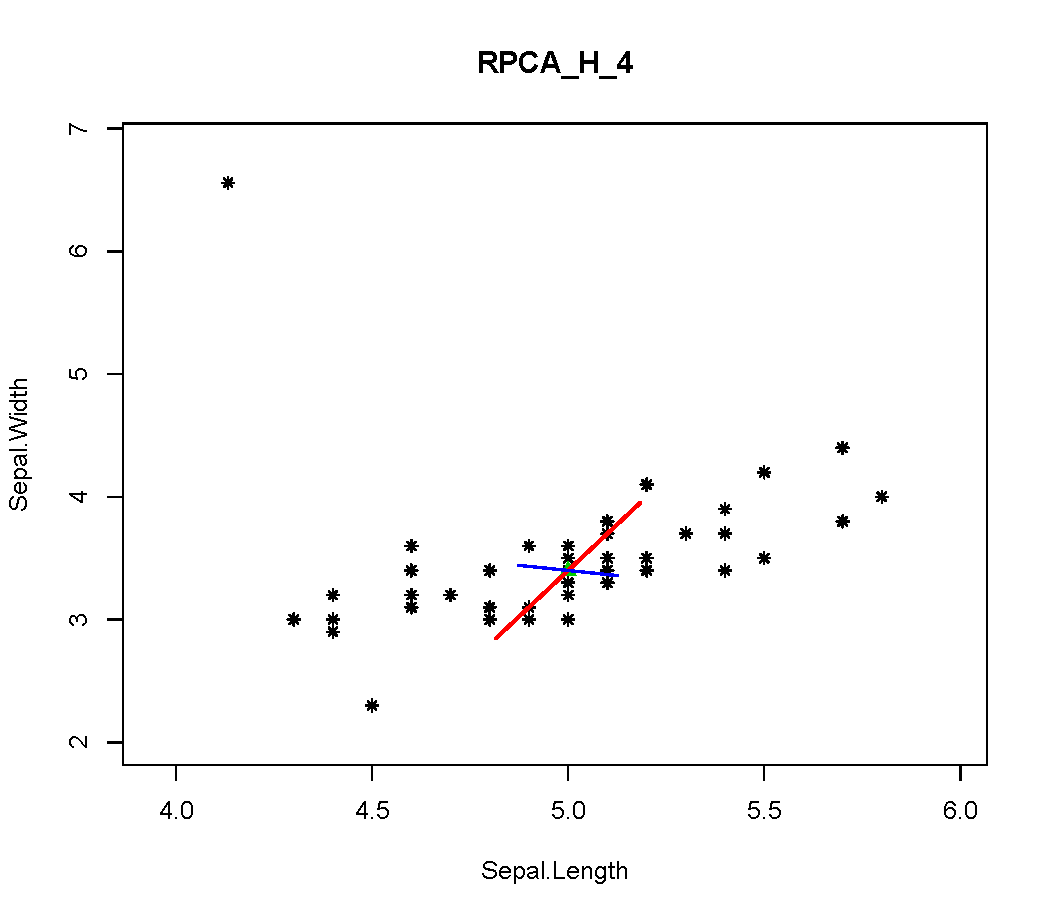
\includegraphics[width=0.3\textwidth]{./RobustPCA_Figures/Iris_Sepal_PCA_Out_H4} \\
\end{tabular}
\end{center}
\caption{The sepal length and width of \textit{Iris Setosa}. The principal components are obtained using 
the function \texttt{robpca} from the library \texttt{rospca}
(upper left panel, denoted by \texttt{RPCA\_H\_0}), 
the function \texttt{rospca} from the library \texttt{rospca} 
(upper middle panel, denoted by \texttt{RPCA\_H\_1}), 
the function \texttt{PCAgrid} from the library \texttt{pcaPP} 
(upper right panel, denoted by \texttt{RPCA\_H\_2}), 
the function \texttt{GSE} from the library \texttt{GSE} 
(lower left panel, denoted by \texttt{GSE}), 
the function \texttt{prcomp.robust} from the library \texttt{mdqc} 
(lower middle panel, denoted by \texttt{Prcomp\_Robust}), 
the function \texttt{SPcaGrid} from the library \texttt{rrcovHD}
(lower right panel, denoted by \texttt{RPCA\_H\_4}). 
}
\label{Figure:PP_PCA}
\end{figure}
%
Performances of these packaged functions vary widely, both in terms of the quality of results and time taken for computations. In Figure~\ref{Figure:PP_PCA}, we report principal components on the Iris sepal data with the single outlier, that was used for the right panel of Figure~\ref{Figure:1}. Roughly, the principal components ought to look like the red and blue lines in the left panel of Figure~\ref{Figure:1}, when a proposed robust PCA method performs well. However, as is evident from Figure~\ref{Figure:PP_PCA}, projection pursuit methods miss this mark: all the methods we explored seem to have issues with either the length of the eigenvectors, or their direction, or both. 

This unsatisfactory performance of PCA using projection pursuits is not a new observation. Similar issues have been noted earlier in \cite{ref:Technometrics05264_Maronna_RCPA} and \cite{ref:EJS111123_Tropp_RPCA}. The latter paper also noted that several of the proposed robust PCA techniques based on projection pursuit ideas are \textit{ad hoc} in nature, involving computations that may require time or computer memory capacity of the order of exponentials in sample size or data dimension, and some may lack underlying statistical theoretical basis.

 In a systematic evaluation of PCA using projection pursuit, \cite{ref:EJS111123_Tropp_RPCA} studied the problem of obtaining the first eigenvector as
\ban 
G_{1, MD} = \arg \max_{| v | = 1} \sum_{i = 1}^{n} | \langle {X}_{i}, v \rangle |.
\ean 
This may be considered a potentially robust alternative to classical PCA, where the first eigenvector is obtained by optimizing $\arg \max_{| v | = 1} \sum_{i = 1}^{n} | \langle {X}_{i}, v \rangle |^{2}$, see \eqref{eq:PCA1}. Thus, $G_{1, MD}$ uses the sample \textit{mean absolute deviation} instead of the sample variance: the use of such a $\ell_{1}$-norm in place of the $\ell_{2}$-norm is often treated as a robust approach in statistics. \citet{ref:EJS111123_Tropp_RPCA} establish that computation of $G_{1, MD}$ is \texttt{NP}-hard, thus proving that many proposed projection pursuit algorithms are infeasible  for routine and regular algorithmic usage on reasonable-sized datasets. However, they also propose an efficient randomized algorithm for an approximation of $G_{1, MD}$. Theorem~2.2 of \cite{ref:EJS111123_Tropp_RPCA} states that for any failure probability $\delta > 0$ and loss factor $\epsilon > 0$, the proposed algorithm provides a unit norm vector $G_{1, MDR}$ such that 
\ban 
\sum_{i = 1}^{n} | \langle {X}_{i}, G_{1, MDR} \rangle |
\geq (1 - \epsilon) {\frac{2}{\pi}} 
\max_{| v | = 1} \sum_{i = 1}^{n} | \langle {X}_{i}, v \rangle |.
\ean
The actual semidefinite programming corresponding to this is polynomial in $n$, and thus 
can be daunting. However, authors provide approaches to solve it efficiently. 

\section{Matrix Decomposition Approaches}
\label{Sec:MatDec_PCA}

In the applied mathematics and machine learning literature, a different kind of development related to robust PCA has been popular. Here, the data matrix is typically decomposed as
\baq
{\vecX} = \vecH_{LR} + \vecR_{Sparse}. 
\label{eq:LRSparse}
\eaq
where $\vecH_{LR}$ is a \textit{low rank matrix}, and $\vecR_{Sparse}$ is a \textit{sparse} matrix. 
This idea originated in \cite{ref:JACM111_Candesetal_RPCA} and \cite{ref:NIPS092080_Wrightetal_RPCA} and is often referred to as \textit{principal component pursuit} (PCP hereafter). Note that \eqref{eq:LRSparse} does not include noise or random components that are routinely used in statistical models and observed in real data. 

There is an immediate identifiability issue: the sparse component $\vecR_{Sparse}$ 
can also be low rank. Consequently, additional conditions are required to ensure identifiability. One such condition is that the low-rank component is \textit{incoherent}, ie, not-sparse. The optimization problem tied to \eqref{eq:LRSparse}  is $\min \bigl[ rank (\vecH) + \lambda | \vecR |_{0} \bigr]$, 
such that  ${\vecX} = \vecH + \vecR$, for some suitable regularization parameter 
$\lambda > 0$, where $| \vecR |_{0}$ is the number of non-zero elements of $\vecR$. 
A computationally viable alternative is
\baq
\min \bigl[  \sum_{i = 1}^{\min{\{n, p\}}} \sigma_{i} (\vecH) 
+ \lambda | \vecR |_{1} \bigr],
\label{eq:PCPursuit}
\eaq
 such that  ${\vecX} = \vecH + \vecR$, where 
$| \vecR |_{1} = \sum_{i = 1}^{n}\sum_{j = 1}^{p} | R_{i j} |$. 
While in typical optimization problems like the above, $\lambda$ is often determined computationally using cross-validation or other methods,  \cite{ref:JACM111_Candesetal_RPCA} 
obtain an exact value for $\lambda$ for any data $\vecX$ in the above framework, which is an interesting result. Other choices of norms for $\vecH$ and/or $\vecR$, using different basis functions for interesting low-rank representations, and several other variations of the above approach have been studied in the past few years. 
The paper \cite{ref:CVIU1422_RPCA_Review}  is a review paper on 
PCP and related matrix decomposition methods for video surveillance, and \cite{ref:ProceedingsIEEE181359_RPCA_Review} is a more recent review paper. In these papers numerous other variations of the original PCP idea are reviewed and evaluated. 

Some variations of matrix decomposition algorithms like the PCP 
are noteworthy from a statistical perspective.
In \cite{ref:TransactionsOnImageProcessing123794_PCA}, the authors argue that the original PCP approach for fitting \eqref{eq:LRSparse}  is computationally expensive, and all computations have to be repeated if additional observations come in. 
Authors propose the variant 
$\min \bigl[  \sum_{i = 1}^{\min{\{n, p\}}} \sigma_{i} (\vecU) 
+ \lambda | \vecR |_{1} \bigr]$ such that ${\vecX} =    {\vecX} \vecU  + \vecR$.
\attention{I need to state what is $U$ here.}
To address the issue that real data is not noise-free, in \cite{ref:IEEEISIT101518_RPCA} the authors propose the optimization problem 
$\min \bigl[ | \vecH |_{*} +  \lambda | \vecR |_{1}$
such that $| \tilde{\vecX} -    \vecH - \vecR |_{F} < \delta$ for some $\delta > 0$. The paper \cite{becker2011tfocs} also has similar ideas. 
In \cite{ref:ICASSP123925_RPCA}, local low-rank structures 
for data on a manifold are used, thus essentially obtaining a union of low-rank subspaces. In \cite{ref:ACISS101_RPCA}, a block sparsity alternative is proposed. Bayesian approaches for PCP are proposed in \cite{ref:TransactionsInImageProcessing113419_PCA_Bayesian, 
ref:IEEETransSignalProciessing123964_RPCA_Bayesian, ref:CSDA17144_RPCA_Bayesian}.


An interesting matrix decomposition proposal comes from \cite{ref:EJS111123_Tropp_RPCA},
who propose the optimization 
$\sum_{i} \sigma_{i} (\vecH) + \lambda \sum_{i} \bigl( \sum_{j =1}^{p} R_{i, j}^{2} \bigr)^{1/2}$ such that ${\vecX} = \vecH + \vecR$, and call it the \textit{low leverage decomposition} (LLD). Here, $\vecR$ may be interpreted as outliers and $\vecH$ as the uncorrupted version of the data, then PCA can then be obtained using $\vecH$. Invariance to choice of observational basis, often considered a critical property of PCA, is available in LLD, but not necessarily for PCP or many of its variants. Other interesting developments related to low-rank matrix representation ideas may be found in
\cite{ref:SIAMJOpt11572_Chandrasekaran_RPCA, ref:NeurIPS11612_RPCA_Ctype, ref:ICML10663_Liu_RPCA, ref:NIPS102496_RPCA_OutlierPursuit, ref:AISTAT14266_RPCA_Gilad, ref:TransactionsOnSignalProcessing125176_PCA, ref:StatScience12450_PCA, ref:IEEETransactionsOnIT123047_PCA, ref:NIPS13404_PCA, ref:TransactionsInInformationTheory13546_PCA, ref:NIPS141107_Netrapalli_PCA, ref:JMLR14749_Lerman_PCA, ref:ICML1455_PCA, vidal2016robust, ref:IEEETransactionsOnSIgnalProcessing192439_PCA, ref:ICML212739_PCA, ref:ICML212341_PCA} and many other places. This area of research has an overwhelming number of papers of varying quality. Several applications of the above framework are listed in the papers above and include video surveillance, face recognition, latent semantic indexing, ranking and collaborative filtering, graph clustering and many more.

While there is an intuitive connection between robust PCA and decomposition of a matrix in low-rank and sparse components, the statistical properties of this framework need further research. This can begin with fixing a population model for the data, clearly defining the principal components, establishing consistency and efficiency results, and also establishing robustness-related results in terms of breakdown properties, influence functions and so on. A major theoretical limitation, as far as most standard data analysis problems are concerned, is the underlying assumption in many (or all) related papers that the ``true'' population is a low-rank structure (that is estimated using $\vecH_{LR}$), anything else in the data is an outlier or at best, a very small perturbation error. This is similar to saying that if $\BX_{i}$'s are iid $N_{p} (\mu, \Sigma)$, then $\Sigma$ is a rank-deficient singular matrix, which is not a practical assumption in many cases.

\begin{figure}
\begin{center}
\begin{tabular}{cc}
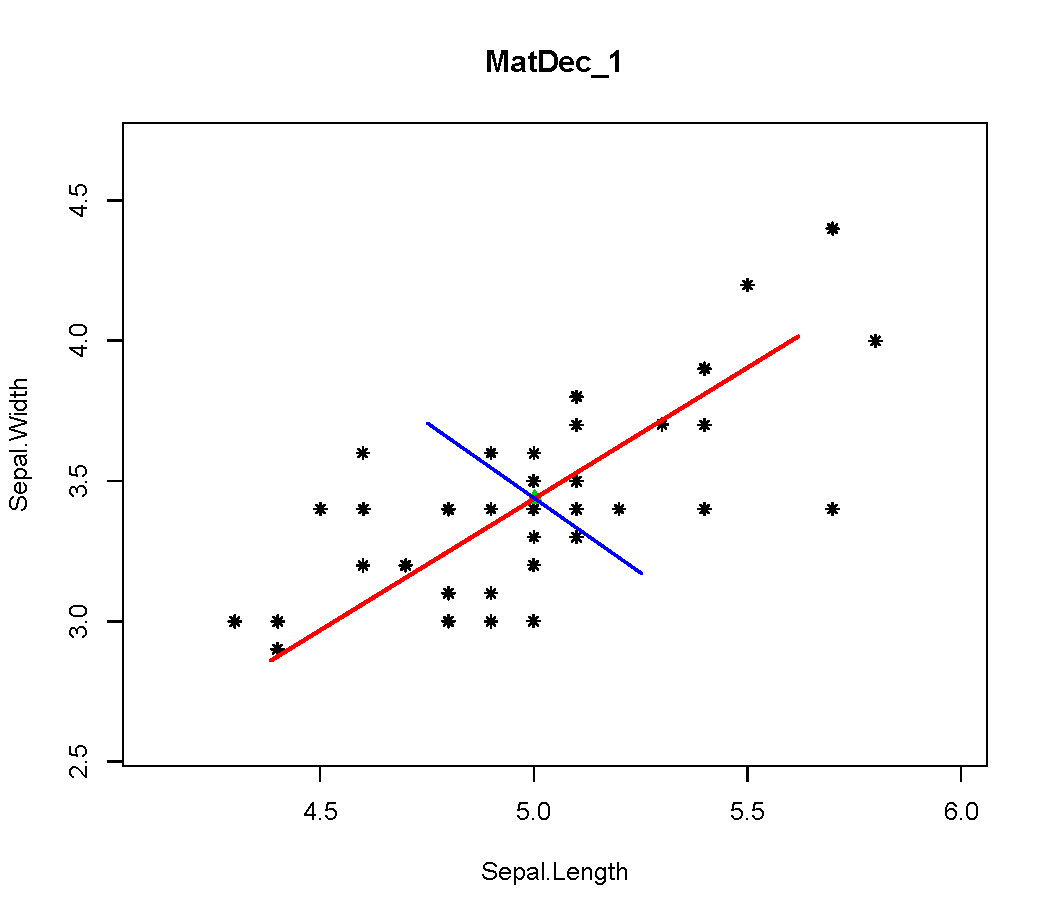
\includegraphics[width=0.49\textwidth]{./RobustPCA_Figures/Iris_Sepal_PCA_Out_MatDec1} &
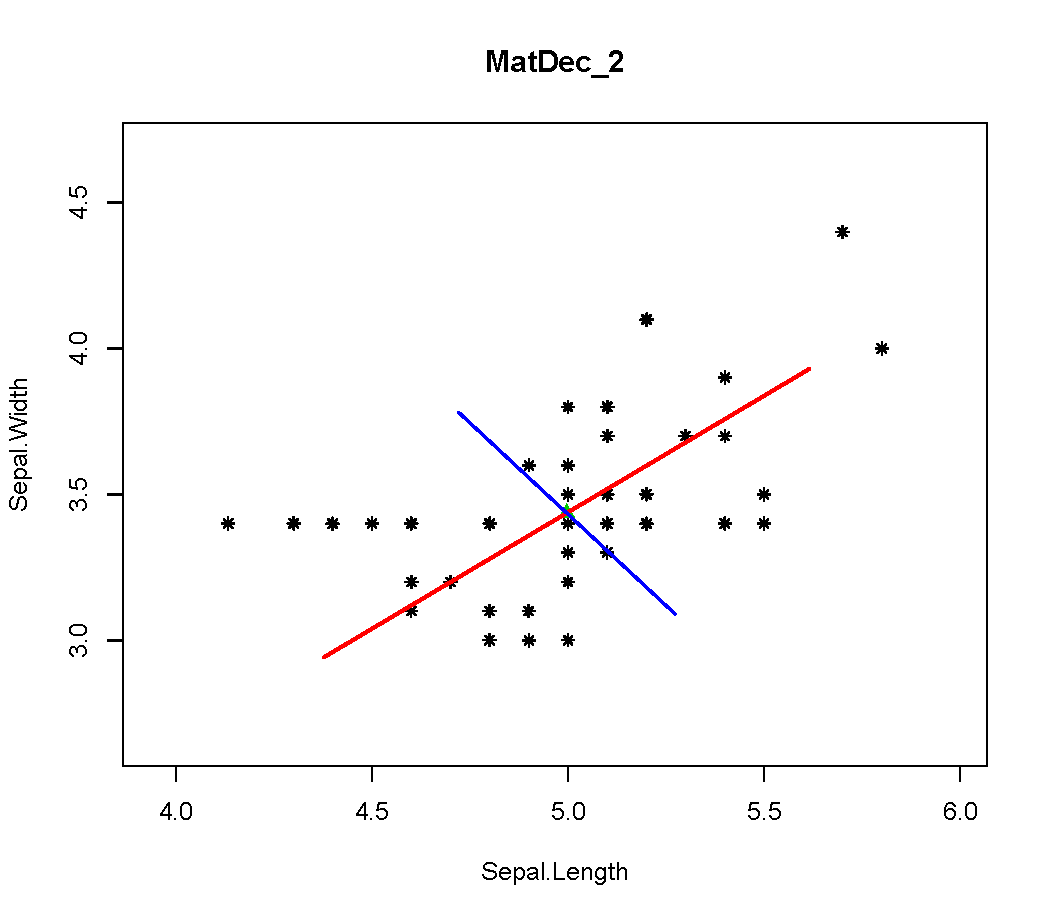
\includegraphics[width=0.49\textwidth]{./RobustPCA_Figures/Iris_Sepal_PCA_Out_MatDec2} \\
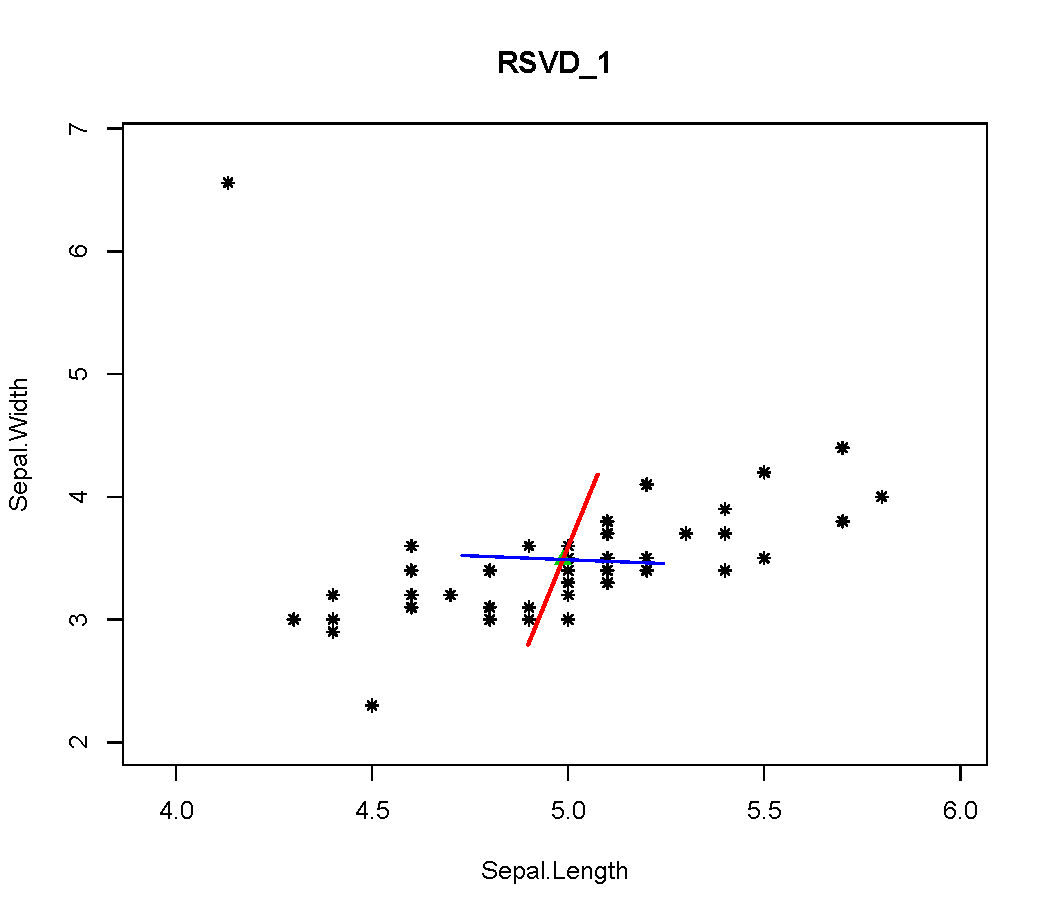
\includegraphics[width=0.49\textwidth]{./RobustPCA_Figures/Iris_Sepal_PCA_Out_RSVD}  &
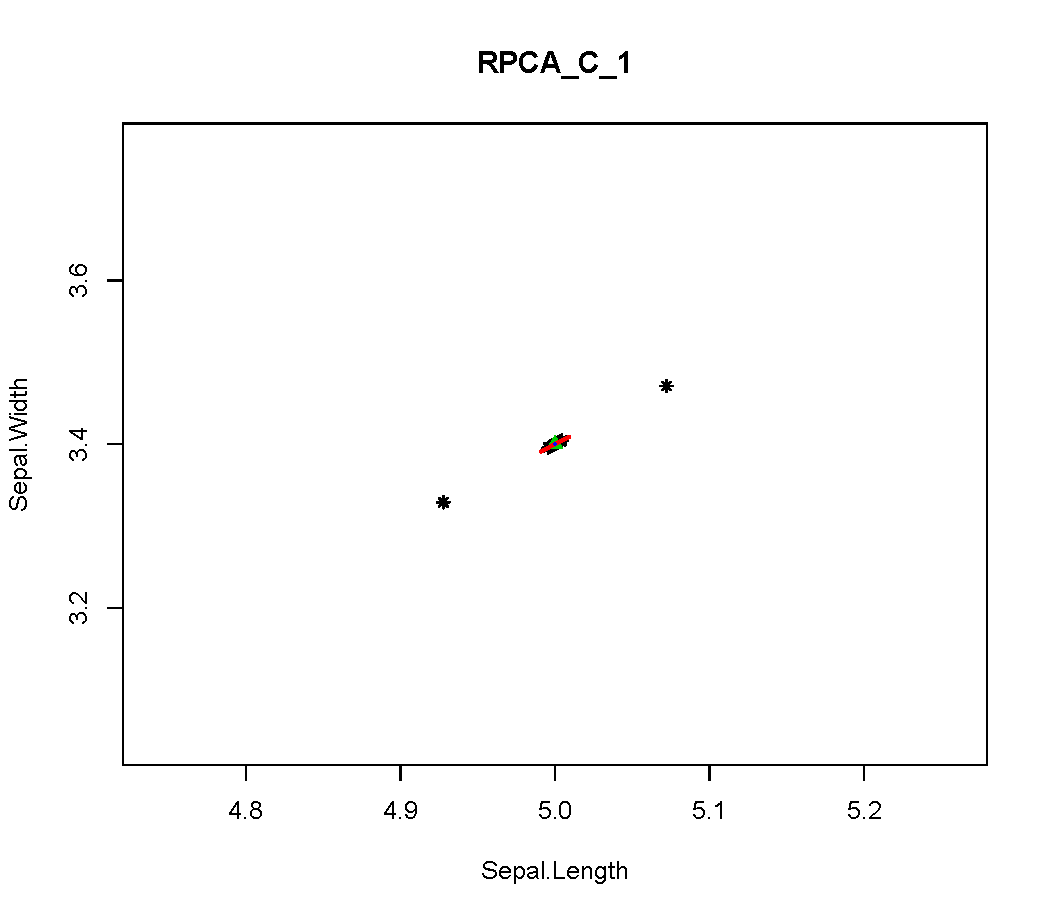
\includegraphics[width=0.49\textwidth]{./RobustPCA_Figures/Iris_Sepal_PCA_Out_C1} \\
\end{tabular}
\end{center}
\caption{The sepal length and width of \textit{Iris Setosa}. The principal components are obtained using 
our own code for PCP
(upper left panel, denoted by \texttt{MatDec\_1}), 
our own code for LLD
(upper left panel, denoted by \texttt{MatDec\_2}), 
the function \texttt{robspca} from the library \texttt{sparsepca} 
(lower left panel, denoted by \texttt{RSVD\_1}), 
the function \texttt{rrpca} from the library \texttt{rsvd}
(lower right panel, denoted by \texttt{C\_1}). 
}
\label{Figure:MatDec_PCA}
\end{figure}

Further algorithmic and software developments on matrix decomposition methods are needed. We were disappointed when searching for readymade software products on matrix decomposition proposals that may be useful for statisticians. Many proposed algorithms are not publicly available as software, and some are claimed to be in repositories that are no longer publicly available. Some available packages and functions failed to work even in the simple Iris Setosa sepal data. We found that the function \texttt{rrpca} in package \texttt{rsvd} to be functional over this data. Several of the downloadable software code  on matrix decompositions fail  to produce reasonable estimates of eigenvalues, eigenvectors or PC-projections, probably because the fundamental framework \eqref{eq:LRSparse} has no room for routine stochasticity in data.  In Figure~\ref{Figure:MatDec_PCA}, we present the principal components on the Iris sepal data with the single outlier, that was used for the right panel of Figure~\ref{Figure:1}. The figures on the upper panels are based on codes we wrote on the PCP and the LLD approaches using ideas similar to \cite{ref:NIPS164152_PCA_SGD}, the bottom panels are based on two \texttt{R} packages. The scatter plot is distorted in all the figures, which is natural,  however, the figures on the bottom panels also have distorted principal components, which is undesirable. 


A related, but considerably different kind of data matrix decomposition technique is reviewed extensively in \cite{ref:ProceedingsIEEE181380_RPCA_Lerman_Review}. Here, the assumption is that many of the $n$ observations lie in a low-dimensional subspace $\cH \subset \BR^{p}$, while other observations are on all of $\BR^{p}$. This is often referred to as the \textit{robust subspace recovery} (RSR) problem.
Here, the goal is recover the low-dimensional subspace $\cH$, which may result in a decomposition of the data as ${\vecX} = \vecH + \vecR$, where the columns of $\vecH$ are expected to span $\cH$, but here $\vecR$ is typically neither sparse, nor expected to be populated by isolated outliers. The above reference provides an extensive literature review with considerable details on RSR, including a rich discussion on its relation to other matrix decomposition approaches and to projection pursuit PCA. Also included are discussions on related regression approaches and several other techniques.

%\attention{Done up to here.}

\section{PCA on (weighted) signs}
\label{Sec:Sign_PCA}

The \textit{generalized sign function} 
 $S : \BR^{p} \to \BR^{p}$ with center $\mu$ is  
 defined as
\baq
S (x; \mu) =  \left\{ 
\begin{array}{ll}
|| x - \mu ||^{-1} ( x - \mu ) &  \text{ if } x \ne \mu, \\
0 & \text{ if } x = \mu.
\end{array}
\right.
\label{eq:GSign}
\eaq
This is the multivariate  generalization of the real-valued 
\textit{sign function}, which
takes the values one, negative one or zero if the point $x \in \BR$ is to the right, left 
or equal $\mu \in \BR$ respectively. This generalized sign function was  
introduced by \cite{ref:JNonpara95201_MottonenOja95}.

The idea of PCA on signs is simple: using a suitable location estimator $\hat{\mu}$, we 
obtain the signs of the observed data $S_{i} = S(\BX_{i}; \hat{\mu})$, and then use the classical PCA on $\{ S_{1}, \ldots, S_{n} \}$. PCA on weighted signs is equally simple: one performs classical PCA on  $\{ Y_{1}, \ldots, Y_{n} \}$, where $Y_{i} = W_{i} S_{i}$ is defined using a suitable weight function $W_{i}$. Note that the classical PCA and the PCA-on-signs can both be treated as special cases of PCA on weighted signs. Also note that it is possible to obtain a (weighted) sample covariance of signs without using a location estimator, using $ \binom{n}{2}^{-1} \sum_{i, j}^{\not=} W_{i, j} || \BX_{i} -  \BX_{j} ||^{-2} (\BX_{i} -  \BX_{j}) (\BX_{i} -  \BX_{j})^{T}$ for appropriate weights $\{ W_{i, j} \}$. The PCS on signs or weighted signs can be obtained from the top eigenvalues/vectors of this matrix. 

PCA-on-signs has been studied in detail, for example in \cite{ref:Test991_RPCA_FPCA, ref:Technometrics05264_Maronna_RCPA, ref:EJS111123_Tropp_RPCA}. All of them found that this approach is viable and convenient method for robust PCA that involves minimal computational burden, and often yields excellent empirical perfomance. \citet{ref:SPL12765_Taskinenetal} established that if the data 
$\{ \BX_{i} \in \BR^{p}: i =1, \ldots, n \}$ are iid from an elliptically symmetric distribution, then the sample eigenvectors from the original data and from its sign transformations are the same, which explains why PCA-on-signs is often an excellent choice for a robust PCA technique.

 \begin{figure}
\begin{center}
\begin{tabular}{cc}
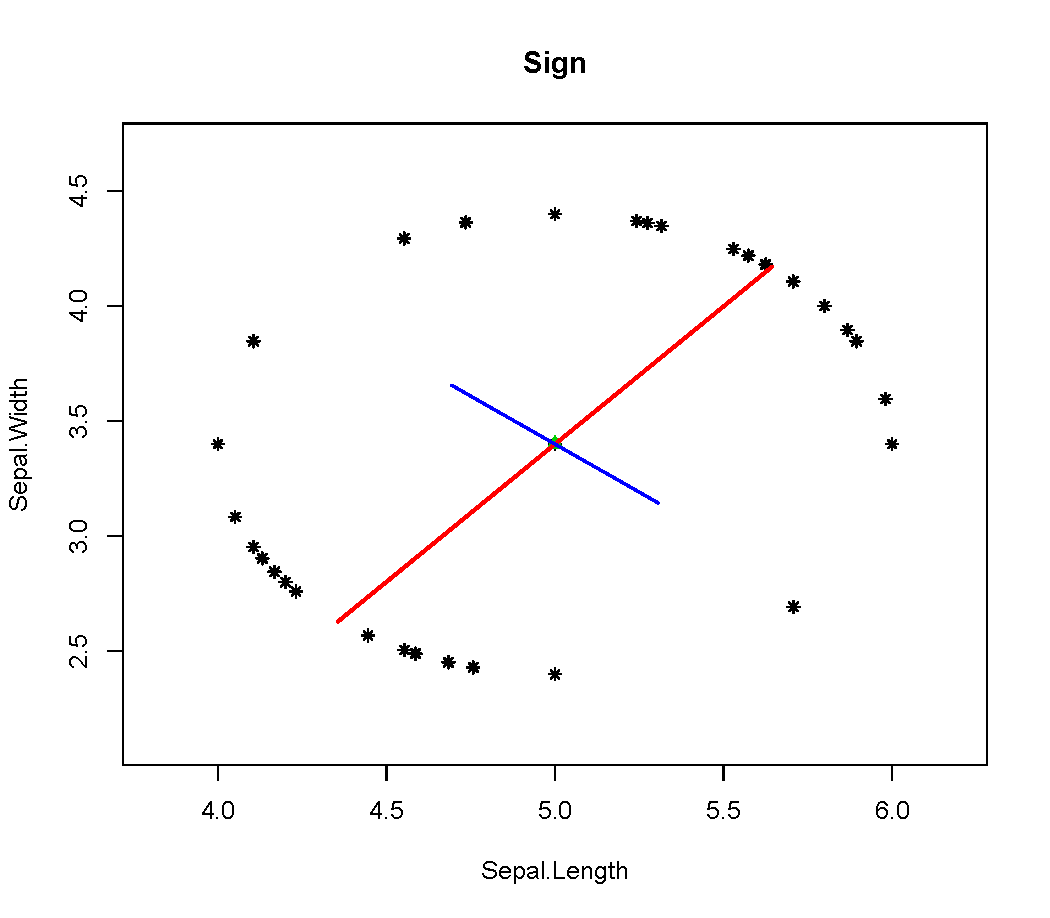
\includegraphics[width=0.49\textwidth]{./RobustPCA_Figures/Iris_Sepal_PCA_Out_Sign} &
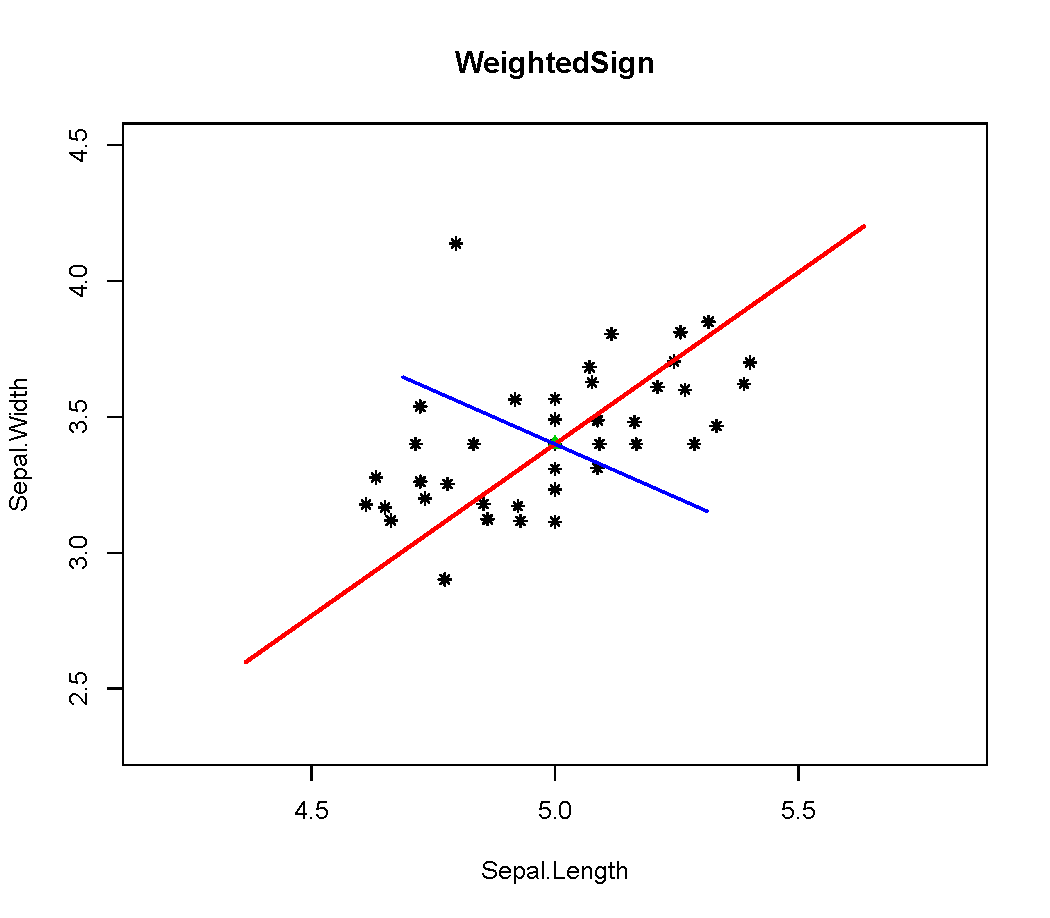
\includegraphics[width=0.49\textwidth]{./RobustPCA_Figures/Iris_Sepal_PCA_Out_WSign} 
\end{tabular}
\end{center}
\caption{The sepal length and width of \textit{Iris Setosa}. The left panel shows the principal components based on generalized signs, computed using the classical PCA algorithm. The right panel is PCA using weighted signs. }
\label{Figure:Sign_PCA}
\end{figure}

However, \cite{majumdar2019weighted} argued that just using the generalized signs may lead to  loss of information and inefficiency. The eigenvector estimates obtained from the covariance matrix of $\{ S_{1}, \ldots, S_{n} \}$ are asymptotically inadmissible \citep{ref:Biometrika14673_MagyarTyler},  and  Tyler's M-estimate of scatter \citep{ref:AoS87234_Tyler} has uniformly lower asymptotic risk, thus confirming the inefficiency observed in \cite{majumdar2019weighted}. \citet{majumdar2019weighted} proposed using classical PCA on  $\{ Y_{i} = W_{i} S_{i}, \ i = 1, \ldots, n \}$, where the weights $W_{i}$ are inverse functions of data depths, that is, the weight of points increase the further they are away from the center $\mu$. The choice $W_{i} = || x - \hat{\mu} ||$ obtains the non-robust classical PCA, while $W_{i} = 1$ obtains the potentially inefficient PCA-on-signs. Empirical evidence presented in \cite{majumdar2019weighted} suggest that a choice of weights, that increase with $|| x - \hat{\mu} ||$ but remain bounded, satisfies robustness objectives while being more efficient than PCA-on-signs. The PCA-on-signs or on weighted signs primarily aim to get reliable estimates of the eigenvectors, and obtaining robust estimators of eigenvalues (and subsequently PCA and PC-projections) are simple steps beyond that. The computational burden of obtaining the weights should be considered while using the PCA-on-weighted-signs method: data-depths may involve intense computations. 

In Figure~\ref{Figure:Sign_PCA} we depict the PCA-on-signs and the PCA-on-weighted-signs  in the left and right panel respectively, for the Iris sepal data with the single outlier.  A coordinatewise median $\hat{\mu}$ is used to center the data, and the weight used is $W_{i} = || x - \hat{\mu} ||/(1 + || x - \hat{\mu} ||)$. This weight does not necessarily satisfy the technical requirements laid out in \cite{majumdar2019weighted}, but is simple computationally. The data scatter is not identical to the original data, as these techniques transform the dataset. As is evident from Figure~\ref{Figure:Sign_PCA}, using PCA-on-signs with or without weights, one can obtain principal components that are robust and accurate. The computational overhead is minimal, and theoretical results are available for iid data from elliptically contoured distributions like the multivariate Gaussian or the multivariate $t$-distributions. Additional theoretical studies, including on the choice of weights, are needed. 

\section{Random projection approaches}
\label{Sec:RanProj_PCA}
The code that we have written for the PCP and LLD methods of Section~\ref{Sec:MatDec_PCA} involved zero-order optimization and stochastic steps. Other randomized algorithms, and in particular random projections and randomly subsetting the data, have been used recently for a variety of tasks related to PCA. The strength of these algorithms lies in their speed and strong theoretical performance guarantees, as well as statistical performance guarantees in some cases. Importantly in high-dimensional problems where sparse PCA may be required, algorithms with stochastic steps have proved to be strong performers \cite{ref:JRSSB20329_PCA_Samworth, ref:Arxiv1712.05630_PCA_Samworth}. Other related studies involving random projections or other randomized steps are in \cite{kaloorazi2016switched, ref:IEEETransactionsOnImageProcessing092230_PCA, qi2012invariance, ref:ICML141341_PCA, mu2011accelerated, ref:ICML11xx_PCA, fischler1981random, ref:JRSSB17959_Samworth, ref:IEEETransactionsOnIT116256_RMT, ref:JAppliedRemoteSensing18015015_PCA, ref:EJS183673_PCA, ref:SIAMJAPPMath20977_Kutz_SPCA}. 

% \begin{figure}
%\begin{center}
%\begin{tabular}{cc}
%\includegraphics[width=0.49\textwidth]{./Iris_Sepal_PCA_Out_RP0} &
%\includegraphics[width=0.49\textwidth]{./Iris_Sepal_PCA_Out_RP1} 
%\end{tabular}
%\end{center}
%\caption{The sepal length and width of \textit{Iris Setosa}. The left panel shows the principal components based on estimating the eigenvectors using random data subsets. 
%The right panel is similar, but with weights associated with the random data subsets. }
%\label{Figure:RP_PCA}
%\end{figure}

 \begin{figure}
\begin{center}
\begin{tabular}{cccc}
\includegraphics[width=0.49\textwidth]{./RobustPCA_Figures/Iris_Sepal_PCA_Out_RP0} &
\includegraphics[width=0.49\textwidth]{./RobustPCA_Figures/Iris_Sepal_PCA_Out_RP1} 
\end{tabular}
\end{center}
\caption{The sepal length and width of \textit{Iris Setosa}. The left panel shows the principal components based on estimating the eigenvectors using random data subsets. 
The right panel is similar, but with weights associated with the random data subsets. }
\label{Figure:RP_PCA}
\end{figure}



In typical statistical problems, the number of outliers or other rogue observations is small, hence if we select a small subset of the data randomly, the probability is high that the selected subset would consist of trustworthy observations only. Such random subsetting of the data may be done repeatedly. We may extract a candidate first eigenvector from each of these random subset of the data, and select (or robustly estimate) the first eigenvector from these candidate eigenvectors. This process may be repeated for any of the principal components. We implemented this algorithm using
PCA-on-signs with and without weights for the robust estimation of the eigenvector from the several candidate eigenvectors obtained from random subsets of the data. Other approaches for robust estimation of eigenvectors could have been used as well, for example those based on medians for data on spheres or related data-depth ideas \cite{ref:EJS14795_MultQuant, ref:AoS921468_LiuSingh_Depth_Spherical}. For weights (when the weighted version the eigenvector from random subsets was used), we simply used the difference between the standard deviations of the first and second principal components, scaled by the standard deviation of the first principal component. This scheme puts greater weight on observations that are closer to the first principal component in angular distance. A thorough and careful study on the choice of weights is needed.
In Figure~\ref{Figure:RP_PCA} we depict the PCs based on these ideas for the Iris sepal data with the single outlier.  This random subsetting and robust estimation algorithm is clearly an excellent performer, and deserves further study.

\section{Other techniques}
\label{Sec:Misc_PCA}
A number of additional methods related to robust PCA have been published. These incude techniques such as the robust covariance matrix estimators
\cite{ref:Biometrics7281_Gnanadesikanetal_RPCA, ref:JASA81354_Devlinetal_RPCA, 
ref:Biometrika00603_CrouxHaesbroeck_RPCA, ref:Bioinformatics071164_PCA}, methods that include outlier identification and removal \cite{dunagan2004optimal, brubaker2009robust}, and many others. 

Many of these methods have been criticized: some employ  elementwise robust estimation of the dispersion matrix, which can result in non-positive sample covariance matrix, many do not have algorithms that can run in polynomial time, and most do not have adequate statistical consistency, efficiency, robustness or computational time and storage complexity guarantees.

%\attention{Done up to here}

\section{Data Experiments}
\label{Sec:DataExpt}
To quantitatively evaluate the performance of different robust PCA techniques, We discuss two data experiments below. First, we consider the \textit{Iris Setosa} sepal data with a single outlier that we have used for illustration throughout this paper, and report on some quantitative measures of performance for several proposed robust PCA algorithms. Then, we compare performances of different robust PCA algorithms on a larger dataset with $n = 7603$ observations and $p = 100$ variables and with $9.2\%$ of the observations containing outliers,.

\subsection{Iris Setosa with outlier data}


% latex table generated in R 3.6.3 by xtable 1.8-4 package
% Mon Sep  6 12:28:53 2021
\begin{table}[ht]
\centering
\begin{tabular}{rrrrr}
  \hline
 & Frobenius & E\_Values & E\_Vectors & Time \\ 
  \hline
Classical & 21.14 & 2.11 & 100.72 & 51.60 \\ 
  Sign & \textbf{2.31} & \textbf{0.03} & \textbf{8.17} & \textbf{16.30} \\ 
  WeightedSign & \textbf{3.45} & \textbf{0.05} & \textrm{13.46} & \textbf{17.90} \\ 
  RP\_PCA\_0 & \textbf{1.36} & \textbf{0.04} & \textbf{5.61} & 78.50 \\ 
  RP\_PCA\_1 & \textbf{4.93} & \textbf{0.11} & 19.92 & 31.40 \\ 
  MatDec\_1 & \textbf{5.87} & \textbf{0.19} & 16.39 & 111.80 \\ 
  MatDec\_2 & 8.51 & 0.45 & 31.94 & 37.00 \\ 
  RPCA\_H\_0 & 18.12 & 4.11 & 16.96 & \textbf{19.00} \\ 
  RPCA\_H\_1 & 20.66 & 6.06 & 28.50 & 58.70 \\ 
  RPCA\_H\_2 & 13.72 & 0.42 & 80.60 & \textbf{18.60} \\ 
  RPCA\_H\_3 & 13.72 & 0.42 & 80.60 & \textbf{15.60} \\ 
  		GSE & 20.01 & 5.38 & \textbf{5.65} & 21.40 \\ 
  Prcomp\_Robust & 151.25 & 40.20 & \textbf{9.76} & 152.60 \\ 
  RPCA\_H\_4 & 16.83 & 2.56 & 80.60 & 25.30 \\ 
  RSVD\_1 & 16.29 & 1.05 & 114.59 & 69.70 \\ 
  RPCA\_C\_1 & 23.61 & 13.08 & \textbf{11.24} & 22.80 \\ 
  RPCA\_Bio\_1 & 21.14 & 46.54 & 181.02 & 23.30 \\ 
   \hline
\end{tabular}
\caption{Performances of different robust PCA methods on the \textit{Iris Setosa} sepal data with a single outlier. Top performing performances in each category are in bold. Values are scaled by 100 for better display.}
\attention{Time in what units? }
\label{Table:1}
\end{table}


We compute the errors in estimation of three related parameters:  variance-covariance matrix, the eigenvalues and the eigenvectors. The estimates of these paramaters from the original \textit{Iris Setosa} sepal data are used as the baseline. We compute the difference from this baseline to the estimates obtained from the various PCA methods applied to the data with an outlier. We use the Frobenius norm ($|A|_{F} = (\sum_{i, j} A_{i, j}^{2})^{1/2}$) for measuring the difference in variance matrix estimators, the standard metric  $ (1 - \langle a, b \rangle^{2} )^{1/2}$ between vectors on a unit hypersphere for distance between eigenvector estimators, and the Euclidean norm for distance between two vectors of eigenvalues. 

We also record the time taken to run each of the robust PCA algorithms, since computation should also be an important performance criterion. The data on these metrics for the methods we evaluated is reported in Table~\ref{Table:1}. Of the seventeen methods listed, fifteen have been described earlier. The projection pursuit technique denoted by RPCA\_H\_3 uses the function \texttt{PCAproj} from the library \texttt{pcaPP}, and the one denoted by RPCA\_Bio\_1 uses the function \texttt{pca} with method \texttt{bpca} (denoting Bayesian PCA) from the library \texttt{pcaMethods}. It can be seen that the PCA-on-signs, PCA on weighted signs, along with the random subsetting methods are the best alternatives by most of the criteria used. The matrix decomposition methods PCP and LLD that we coded in MatDec\_1 and MatDec\_2 are also quite competitive. Projection pursuit methods tend to make large errors in estimating eigenvectors, which is arguably a more serious issue. We experimented with  the other species in the Iris dataset and  other combinations of outliers: overall, the above message remains consistent. 
\attention{Mention about other datasets in the conclusions.}


\subsection{Image Data}




 \begin{figure}
\begin{center}
\begin{tabular}{ccccc}
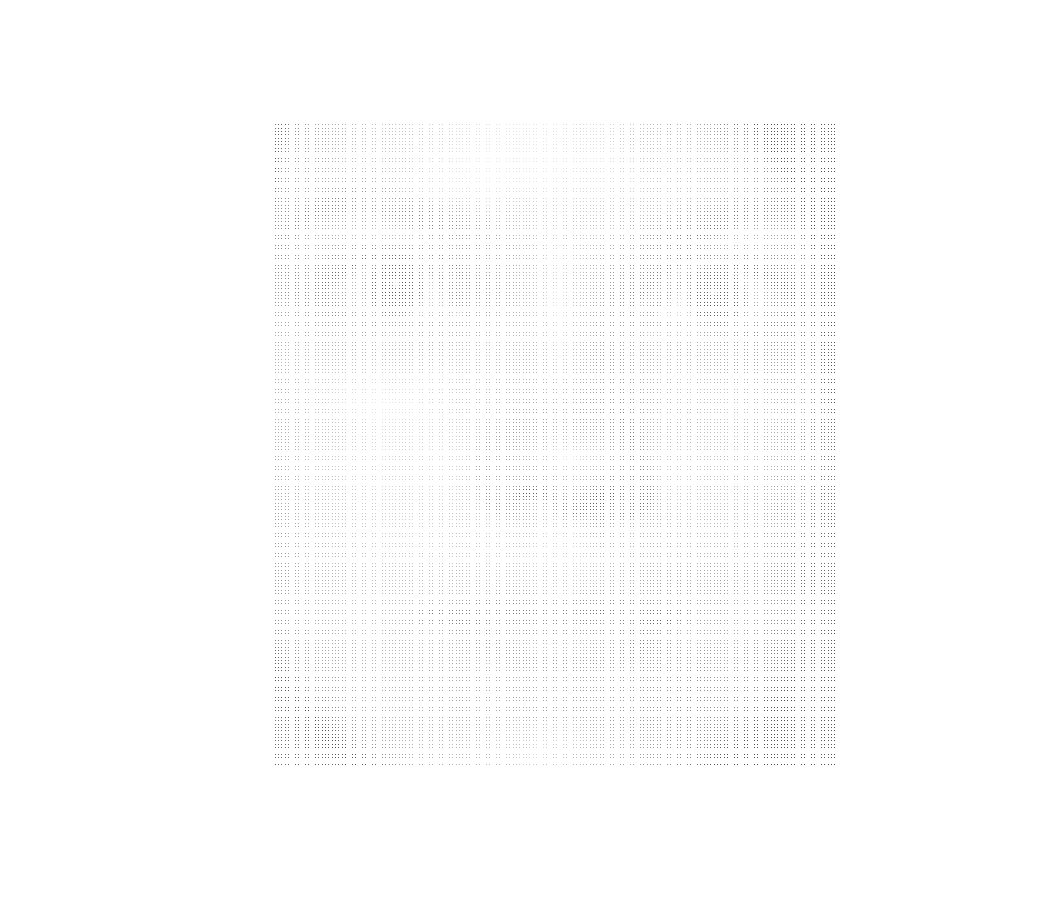
\includegraphics[width=0.19\textwidth]{./RobustPCA_Figures/Yale28_Orig_FullImage} &
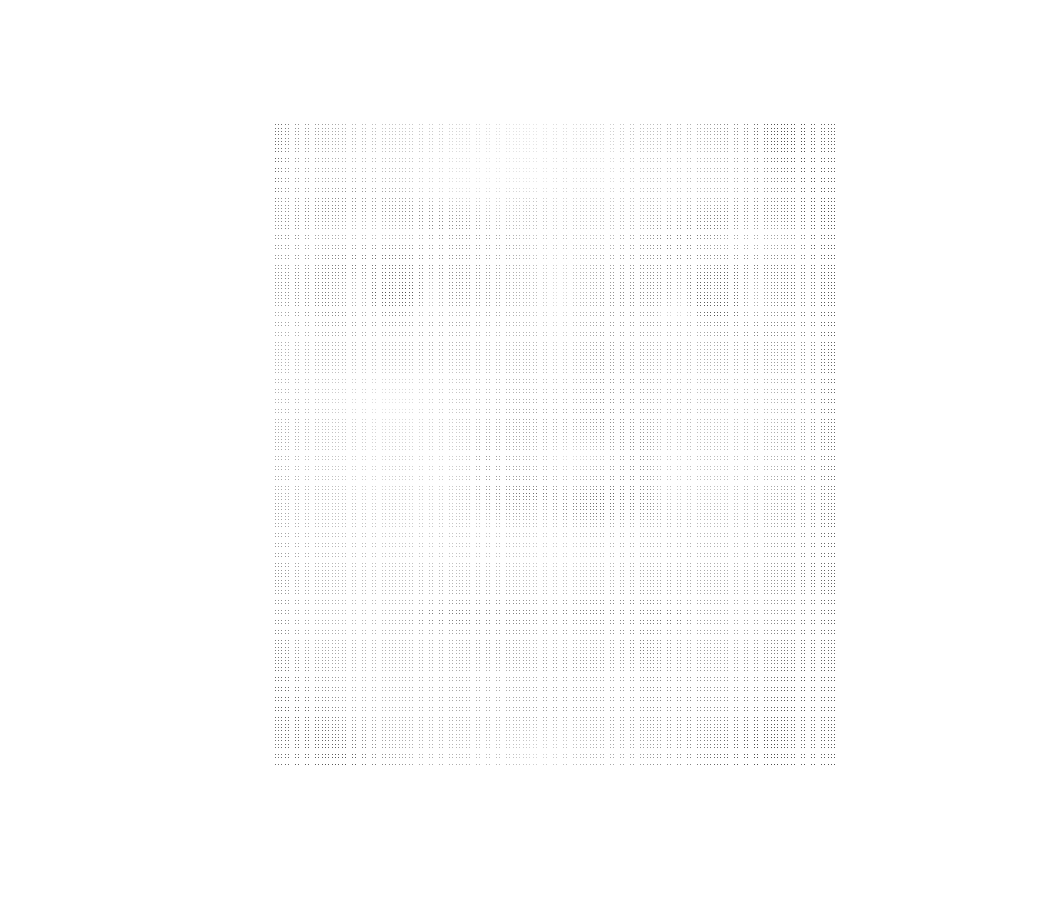
\includegraphics[width=0.19\textwidth]{./RobustPCA_Figures/Yale28_Orig_PC10_Classical} &

\includegraphics[width=0.19\textwidth]{./RobustPCA_Figures/Yale28_Orig_PC10_WSign} &

\includegraphics[width=0.19\textwidth]{./RobustPCA_Figures/Yale28_Orig_PC10_RP1} &

\includegraphics[width=0.19\textwidth]{./RobustPCA_Figures/Yale28_Orig_PC10_MatDec1} 
\\

\includegraphics[width=0.19\textwidth]{./RobustPCA_Figures/Yale28_Orig_PC10_MatDec2} &

\includegraphics[width=0.19\textwidth]{./RobustPCA_Figures/Yale28_Orig_PC10_H2} &

\includegraphics[width=0.19\textwidth]{./RobustPCA_Figures/Yale28_Orig_PC10_H3} &

\includegraphics[width=0.19\textwidth]{./RobustPCA_Figures/Yale28_Orig_PC10_RSVD} &

\includegraphics[width=0.19\textwidth]{./RobustPCA_Figures/Yale28_Orig_PC10_C1} 
\\

\includegraphics[width=0.19\textwidth]{./RobustPCA_Figures/Yale28_Noise3_PC10_MatDec1} &

\includegraphics[width=0.19\textwidth]{./RobustPCA_Figures/Yale28_Noise3_PC10_MatDec2} &

\includegraphics[width=0.19\textwidth]{./RobustPCA_Figures/Yale28_Noise3_PC10_C1} &

\includegraphics[width=0.19\textwidth]{./RobustPCA_Figures/Yale28_Noise6_PC10_MatDec1} &

\includegraphics[width=0.19\textwidth]{./RobustPCA_Figures/Yale28_Noise6_PC10_MatDec2} 
\\
\end{tabular}
\end{center}
\caption{Illustrative example from the  extended Yale Face Database B. In the top row leftmost image is the original data, second to fifth figures are the reconstructions using the top 10 principal components using the classical PCA, PCA-on-sign with weights, PCA using random subsetting and weights (RP\_PCA\_1) and the matrix decomposition method MatDec\_1. In the second row, from left to right, are the the reconstructions using the top 10 principal components on the original data using the matrix decomposition method MatDec\_2, projection pursuit methods RPCA\_H\_2 and RPCA\_H\_3, and matrix decomposition methods  RSVD\_1 and RPCA\_C\_1. In the last row, the first three images are from case ($iv$) with contamination in 10\% randomly selected rows, using matrix decomposition methods MatDec\_1, MatDec\_2 and RPCA\_C\_1.  The last two images are from case ($vii$) where 10\% of rows, columns as well as random pixels were contaminated, and matrix decomposition methods MatDec\_1 and MatDec\_2 used.
\attention{The figures need to be resized and brought to same size, without bezel.}
}
\label{Figure:Yale}
\end{figure}

\begin{table}[ht]
\centering
\begin{tabular}{c|rrrrr}
  \hline
Noise case & Method & Frobenius (x$10^4$) & E\_Values & E\_Vectors & Time \\ 
  \hline
& Classical & 0.00 & 0.00 & 0.00 & 0.23 \\ 
&   Sign & 0.49 & 4.42 & 5.50 & 0.16 \\ 
&   WeightedSign & 0.31 & 2.89 & 3.50 & 0.23 \\ 
&   RP\_PCA\_0 & 0.57 & 8.83 & 5.67 & 13.33 \\ 
&   RP\_PCA\_1 & 0.55 & 4.06 & 6.00 & 13.37 \\ 
(i) None &   MatDec\_1 & 2.23 & 1084.06 & 7.20 & 431.44 \\ 
&   MatDec\_2 & 2.22 & 1062.06 & 6.99 & 220.98 \\ 
&   RPCA\_H\_2 & 3.03 & 946.91 & 9.26 & 4.98 \\ 
&   RPCA\_H\_3 & 2.37 & 297.41 & 8.07 & 0.19 \\ 
&   RSVD\_1 & 4.20 & 1285.54 & 3.97 & 17.21 \\ 
&   RPCA\_C\_1 & 3.53 & 1198.95 & 2.69 & 0.93 \\ 
   \hline
& Classical & 0.89 & 127.57 & 6.73 & 0.38 \\ 
&   Sign & 0.93 & 108.50 & 6.92 & 0.17 \\ 
&   WeightedSign & 0.92 & 115.33 & 6.83 & 0.42 \\ 
&   RP\_PCA\_0 & 1.27 & 120.76 & 8.51 & 16.15 \\ 
&   RP\_PCA\_1 & 1.21 & 113.20 & 8.25 & 16.51 \\ 
(ii) isolated &   MatDec\_1 & 1.85 & 583.98 & 6.96 & 414.99 \\ 
&   MatDec\_2 & 1.83 & 574.64 & 6.96 & 238.36 \\ 
&   RPCA\_H\_2 & 3.27 & 1083.77 & 9.36 & 6.33 \\ 
&   RPCA\_H\_3 & 2.00 & 416.77 & 7.86 & 0.19 \\ 
&   RSVD\_1 & 1.85 & 427.56 & 6.82 & 3.08 \\ 
&   RPCA\_C\_1 & 3.33 & 1143.41 & 3.90 & 1.08 \\ 
   \hline
& Classical & 1.63 & 930.03 & 8.58 & 0.28 \\ 
&   Sign & 1.63 & 894.81 & 8.57 & 0.32 \\ 
&   WeightedSign & 1.62 & 896.19 & 8.57 & 0.21 \\ 
&   RP\_PCA\_0 & 1.73 & 860.89 & 8.79 & 16.46 \\ 
&   RP\_PCA\_1 & 1.81 & 917.67 & 8.82 & 16.74 \\ 
(iv) row &   MatDec\_1 & 1.84 & 448.63 & 6.53 & 442.63 \\ 
&   MatDec\_2 & 1.88 & 487.93 & 6.60 & 188.08 \\ 
&   RPCA\_H\_2 & 4.23 & 3877.72 & 9.71 & 5.48 \\ 
&   RPCA\_H\_3 & 2.80 & 1975.23 & 9.01 & 0.37 \\ 
&   RSVD\_1 & 3.62 & 677.44 & 8.85 & 13.96 \\ 
&   RPCA\_C\_1 & 2.96 & 821.62 & 4.84 & 1.21 \\ 
   \hline
& Classical & 2.85 & 2527.61 & 8.77 & 0.47 \\ 
&   Sign & 2.34 & 1707.04 & 8.61 & 0.14 \\ 
&   WeightedSign & 2.40 & 1782.09 & 8.59 & 0.41 \\ 
&   RP\_PCA\_0 & 2.46 & 1744.60 & 9.09 & 14.86 \\ 
&   RP\_PCA\_1 & 2.63 & 1906.70 & 9.25 & 12.95 \\ 
(vii) row, column &   MatDec\_1 & 2.23 & 863.75 & 8.69 & 398.32 \\ 
and isolated &   MatDec\_2 & 2.23 & 888.69 & 8.66 & 199.15 \\ 
&   RPCA\_H\_2 & 4.20 & 3538.45 & 9.77 & 6.11 \\ 
&   RPCA\_H\_3 & 2.56 & 1841.82 & 9.01 & 0.22 \\ 
&   RSVD\_1 & 2.93 & 1921.84 & 8.78 & 2.93 \\ 
&   RPCA\_C\_1 & 3.10 & 1516.37 & 8.69 & 1.06 \\ 
   \hline
\end{tabular}
\caption{Comparative performances of different robust PCA techniques in one image from the extended Yale Face Database B, for different noise scenarios.}
\label{Table:Image_Noise}
\end{table}

% % latex table generated in R 3.6.3 by xtable 1.8-4 package
% % Sun Oct 10 17:58:35 2021
% \begin{table}[ht]
% \centering
% \begin{tabular}{rrrrr}
%   \hline
%  & Frobenius & E\_Values & E\_Vectors & Time \\ 
%   \hline
% Classical & 0.00 & 0.00 & 0.00 & 0.23 \\ 
%   Sign & 0.49 & 4.42 & 5.50 & 0.16 \\ 
%   WeightedSign & 0.31 & 2.89 & 3.50 & 0.23 \\ 
%   RP\_PCA\_0 & 0.57 & 8.83 & 5.67 & 13.33 \\ 
%   RP\_PCA\_1 & 0.55 & 4.06 & 6.00 & 13.37 \\ 
%   MatDec\_1 & 2.23 & 1084.06 & 7.20 & 431.44 \\ 
%   MatDec\_2 & 2.22 & 1062.06 & 6.99 & 220.98 \\ 
%   RPCA\_H\_2 & 3.03 & 946.91 & 9.26 & 4.98 \\ 
%   RPCA\_H\_3 & 2.37 & 297.41 & 8.07 & 0.19 \\ 
%   RSVD\_1 & 4.20 & 1285.54 & 3.97 & 17.21 \\ 
%   RPCA\_C\_1 & 3.53 & 1198.95 & 2.69 & 0.93 \\ 
%   \hline
% \end{tabular}
% \caption{Comparative performances of different robust PCA techniques in one image from the extended Yale Face Database B. The second column is scaled by 10000 for clarity.}
% \label{Table:Image_Noise0}
% \end{table}
% latex table generated in R 3.6.3 by xtable 1.8-4 package
% Sun Oct 10 18:23:30 2021
% \begin{table}[ht]
% \centering
% \begin{tabular}{rrrrr}
%   \hline
%  & Frobenius & E\_Values & E\_Vectors & Time \\ 
%   \hline
% Classical & 0.89 & 127.57 & 6.73 & 0.38 \\ 
%   Sign & 0.93 & 108.50 & 6.92 & 0.17 \\ 
%   WeightedSign & 0.92 & 115.33 & 6.83 & 0.42 \\ 
%   RP\_PCA\_0 & 1.27 & 120.76 & 8.51 & 16.15 \\ 
%   RP\_PCA\_1 & 1.21 & 113.20 & 8.25 & 16.51 \\ 
%   MatDec\_1 & 1.85 & 583.98 & 6.96 & 414.99 \\ 
%   MatDec\_2 & 1.83 & 574.64 & 6.96 & 238.36 \\ 
%   RPCA\_H\_2 & 3.27 & 1083.77 & 9.36 & 6.33 \\ 
%   RPCA\_H\_3 & 2.00 & 416.77 & 7.86 & 0.19 \\ 
%   RSVD\_1 & 1.85 & 427.56 & 6.82 & 3.08 \\ 
%   RPCA\_C\_1 & 3.33 & 1143.41 & 3.90 & 1.08 \\ 
%   \hline
% \end{tabular}
% \caption{Comparative performances of different robust PCA techniques in one image from the extended Yale Face Database B, with 10\% of the pixel values replaced by random contaminants. The second column is scaled by 10000 for clarity. }
% \label{Table:Image_Noise1}
% \end{table}
% % latex table generated in R 3.6.3 by xtable 1.8-4 package
% % Sun Oct 10 18:47:57 2021
% \begin{table}[ht]
% \centering
% \begin{tabular}{rrrrr}
%   \hline
%  & Frobenius & E\_Values & E\_Vectors & Time \\ 
%   \hline
% Classical & 1.63 & 930.03 & 8.58 & 0.28 \\ 
%   Sign & 1.63 & 894.81 & 8.57 & 0.32 \\ 
%   WeightedSign & 1.62 & 896.19 & 8.57 & 0.21 \\ 
%   RP\_PCA\_0 & 1.73 & 860.89 & 8.79 & 16.46 \\ 
%   RP\_PCA\_1 & 1.81 & 917.67 & 8.82 & 16.74 \\ 
%   MatDec\_1 & 1.84 & 448.63 & 6.53 & 442.63 \\ 
%   MatDec\_2 & 1.88 & 487.93 & 6.60 & 188.08 \\ 
%   RPCA\_H\_2 & 4.23 & 3877.72 & 9.71 & 5.48 \\ 
%   RPCA\_H\_3 & 2.80 & 1975.23 & 9.01 & 0.37 \\ 
%   RSVD\_1 & 3.62 & 677.44 & 8.85 & 13.96 \\ 
%   RPCA\_C\_1 & 2.96 & 821.62 & 4.84 & 1.21 \\ 
%   \hline
% \end{tabular}
% \caption{Comparative performances of different robust PCA techniques in one image from the extended Yale Face Database B, with pixel values in 10\% of the rows replaced by random contaminants. The second column is scaled by 10000 for clarity.}
% \label{Table:Image_Noise3}
% \end{table}
% % latex table generated in R 3.6.3 by xtable 1.8-4 package
% % Sun Oct 10 20:52:30 2021
% \begin{table}[ht]
% \centering
% \begin{tabular}{rrrrr}
%   \hline
%  & Frobenius & E\_Values & E\_Vectors & Time \\ 
%   \hline
% Classical & 2.85 & 2527.61 & 8.77 & 0.47 \\ 
%   Sign & 2.34 & 1707.04 & 8.61 & 0.14 \\ 
%   WeightedSign & 2.40 & 1782.09 & 8.59 & 0.41 \\ 
%   RP\_PCA\_0 & 2.46 & 1744.60 & 9.09 & 14.86 \\ 
%   RP\_PCA\_1 & 2.63 & 1906.70 & 9.25 & 12.95 \\ 
%   MatDec\_1 & 2.23 & 863.75 & 8.69 & 398.32 \\ 
%   MatDec\_2 & 2.23 & 888.69 & 8.66 & 199.15 \\ 
%   RPCA\_H\_2 & 4.20 & 3538.45 & 9.77 & 6.11 \\ 
%   RPCA\_H\_3 & 2.56 & 1841.82 & 9.01 & 0.22 \\ 
%   RSVD\_1 & 2.93 & 1921.84 & 8.78 & 2.93 \\ 
%   RPCA\_C\_1 & 3.10 & 1516.37 & 8.69 & 1.06 \\ 
%   \hline
% \end{tabular}
% \caption{Comparative performances of different robust PCA techniques in one image from the extended Yale Face Database B, with pixel values in 10\% of the rows, 10\% of the columns and 10\% randomly chosen other pixels replaced by random contaminants. The second column is scaled by 10000 for clarity.}
% \label{Table:Image_Noise6}
% \end{table}


Our second example is based on images from the extended Yale Face Database B \citep{ref:IEEEPAMI01643_PCA,ref:PAMI05684_PCA}. We experimented with several images of several individuals from this repository, and report here in detail the analysis for one of the images for individual~\#-28. The generic pattern of the results for all other images resemble those presented below. 
%For the results displayed in tables below, the corresponding numbers for many other cases we analyzed were within 90-110\% of the reported here, 
All the images contain grey-level values in each pixel in a $192 \times 168$ grid, scaled to be in the interval $[0, 1]$, thus this is an example where the data is known to be bounded. We consider seven different distortions of the images:
%
\begin{enumerate}[label=\roman*),leftmargin=*]
    \item No noise added to images.
    \item Binary speckle noise: randomly selected pixels are assigned values 0 or 1 with equal probability,
    \item Uniform speckle noise: randomly selected pixels are assigned values drawn iid from $\text{Unif}(0,1)$.
    \item Binary speckle noise in all pixels of randomly selected rows.
    \item Binary speckle noise in all pixels of randomly selected columns.
    \item Binary speckle noise in all pixels of randomly selected rows and columns.
    \item Binary speckle noise in all pixels of randomly selected rows and columns, as well as randomly selected isolated pixels.
\end{enumerate}
%
These cases represent various kinds of contamination of the data, and different levels of contamination as well. For brevity, we present results for the situation where 10\% of pixels, rows and columns were randomly selected for contamination, from only cases $i$, $ii$, $iv$ and $vii$. We consider the top 10 eigenvalue-eigenvectors from the unaltered, original data to construct performance metric baselines, and use the top 10 robust eigenvalue-eigenvectors obtained from each method for comparison. When an image is reconstructed from the top $k$ principal components, the clarity and resemblance of it to the original image are sensitive to the choice of $k$. However, visually from several examples from the extended Yale Face Database B, it seems that a minimum of 5 principal components are needed and choosing more than 20 principal components seems to lead to minor improvements, hence we selected $k =10$ for the present illustrative example. The comparative performances of the robust PCA methods do not seem to depend on the choice of $k$. 

We present the numeric data from cases $i$, $ii$, $iv$ and $vii$ in Table~\ref{Table:Image_Noise}. We first discuss the case where there is no noise (case $i$), and the first 10 principal components are computed using a variety of robust PCA methods. Methods not listed in Table~\ref{Table:Image_Noise} failed to function in this dataset, and generated errors. It can be seen that in this noise-free case, the PCA-on-signs, PCA-on-signs with weights, and the two random subsetting PCA methods performed extremely well. Other methods were also reasonable performers, considering the fact that the distance between the baseline eigenvalues and their robust estimates are scaled by $10^{4}$ for clarity. The two matrix decomposition techniques we coded, MatDec\_1 and MatDec\_2  for PCP and LLD respectively, needed considerably more computation time compared to other methods. In the case where 10\% of randomly selected pixel-values replaced with either  zero or one  (case $ii$), from Table~\ref{Table:Image_Noise} we see that the classical PCA, the two PCA-on signs, and the two random subsetting methods performed better than other methods, while the projection pursuit method RPCA\_H\_2 and the matrix decomposition method RPCA\_C\_1 performing quite poorly. 

In the case  where the pixel values from 10\% randomly selected rows were replaced by either zero or one and in the case where pixel values from 10\% randomly selected rows, as well as 10\% randomly selected columns and an additional 10\% randomly selected pixels from all over the image were replaced by either zero or one  (case $vii$), all methods encounter difficulties. However, the matrix decomposition methods MatDec\_1 and MatDec\_2 perform better than other techniques (third and fourth sections of Table~\ref{Table:Image_Noise}). 

In Figure~\ref{Figure:Yale} we present visual depiction of the image under study and its reconstruction from various techniques. In the top row of Figure~\ref{Figure:Yale}, the leftmost image is the original data, and the second to fifth figures are the reconstructions using the top 10 principal components using the classical PCA, PCA-on-sign with weights, PCA using random subsetting and weights (RP\_PCA\_1) and the matrix decomposition method MatDec\_1. In the second row, from left to right, are the the reconstructions using the top 10 principal components on the original data using the matrix decomposition method MatDec\_2, projection pursuit methods RPCA\_H\_2 and RPCA\_H\_3, and matrix decomposition methods  RSVD\_1 and RPCA\_C\_1. We did not include images from PCA-on-sign and RP\_PCA\_0 since these were visually very similar to those from PCA-on-sign with weights and  RP\_PCA\_1 respectively. It can be easily seen that the reconstructions from RPCA\_H\_3 and RPCA\_C\_1 are extremely poor. 

 In the last row, the first three images are from case ($iv$) with contamination in 10\% randomly selected rows, using matrix decomposition methods MatDec\_1, MatDec\_2 and RPCA\_C\_1.  The last two images are from case ($vii$) where 10\% of rows, columns as well as random pixels were contaminated, and matrix decomposition methods MatDec\_1 and MatDec\_2 used. Visually, the presence of a human face can be detected in the images obtained using MatDec\_1 and MatDec\_2, but not from the image obtained using RPCA\_C\_1.
  We do not show the reconstructions from other methods for brevity, they are generally poorer than those obtained by MatDec\_1 or MatDec\_2, but a human face can still be discerned. 

This example is illustrative of data in moderate dimensions, where noise and contamination is bounded. Many robust PCA methods are motivated by their possible use in image analyses, and it seems that there us some evidence that matrix decomposition methods might perform better than other techniques in the presence of considerable amount of contamination. However, the the PCA-on-signs and random subsetting, with or without weights, remain strong competitors at all levels of noise. More studies on matrix decomposition techniques and further software developments are required.

\clearpage
\subsection{MNIST data with outliers}
We consider the modified version of the MNIST data, proposed in \cite{ref:ICDM14698_PCA} and used as one of the benchmark datasets for studies on outliers from \url{http://odds.cs.stonybrook.edu/}. This  data has $n = 7603$ observations and $p = 100$ variables, and and 9.2\% of the data may be considered outliers. To accentuate the noise we added iid standard Cauchy random variables to each outlying  observation. 
 %
 \begin{table}[t]
\centering
\begin{tabular}{rrrrr}
  \hline
 & Frobenius & E\_Values & E\_Vectors & Time \\ 
  \hline
Classical & 37.08 & 5117.46 & 39.80 & 0.52 \\ 
  Sign & 1.90 & 9.53 & 27.16 & 5.74 \\ 
  WeightedSign & 1.90 & 9.50 & 27.15 & 15.38 \\ 
  RP\_PCA\_0 & 1.87 & 6.75 & 30.77 & 41.26 \\ 
  RP\_PCA\_1 & 1.91 & 6.81 & 30.32 & 41.90 \\ 
  RPCA\_H\_2 & 7.65 & 352.57 & 36.33 & 120.40 \\ 
  RPCA\_H\_3 & 4.57 & 148.55 & 31.48 & 184.42 \\ 
  MatDec\_2 & 15.52 & 837.13 & 39.54 & 1036.33 \\ 
MatDec\_1 & 16.00 & 837.00 & 40.00 & 3926.00 \\ 
  RSVD\_1 & 8687915.00 & 3923401243.00 & 40.00 & 2.00 \\ 
  RPCA\_C\_1 & 269712.00 & 88589972.00 & 38.00 & 8.00 \\ 
   \hline
\end{tabular}
\caption{Robust PCA methods performances on the MNIST data with outliers. 
Methods not listed here generated errors and did not successfully run on this data. The Frobenius norm is scaled by $10^{-4}$ for clarity of presentation.}
\label{Table:2}
\end{table}
%
 The results of the robust PCA techniques on this relatively large-sized and high-dimensional data is reported in Table~\ref{Table:2}. We have used the estimated eigenvalues and eigenvectors from the non-outlier observations to generate the baseline to use for comparing the performances of the robust PCA methods. The methods not listed in Table~\ref{Table:2} failed to function in this dataset, and generated errors. It can be seen that in this medium/large size dataset, the  PCA-on-signs, PCA on weighted signs, and the random subsetting methods have again performed very well, in terms of all the criteria we used. Two projection pursuit approaches, RPCA\_H\_2 and RPCA\_H\_3 that respectively use the functions \texttt{PCAgrid} and \texttt{PCAproj} from the library \texttt{pcaPP}, have done comparably well in terms of estimating the eigenvectors, perhaps acceptably in terms of the dispersion matrix but not so in terms of the eigenvalues. The matrix decomposition methods that we coded were far less satisfactory, and both the LLD approach (MatDec\_2) and PCP  approach (MatDec\_1) took a lot of computation time, with the LLD approach being distinctly better in terms of computational time, and marginally better in terms of statistical performance. The packaged matrix decomposition methods were disastrous in their performances in every metric, but were fast.

\section{Conclusion}
\label{Sec:Conclusion}
We have reviewed several  proposed methods for robust PCA, spanning many decades of work from different groups of researchers. The earlier generation of research in this topic, often using projection pursuit techniques,  concentrated more on intuitive strategies and fixes that were workable on small datasets. In the age of modern computing, where problems routinely require analyzing vast amounts of data in an automated way, many new robust PCA strategies were put forward and seem to produce reasonable results in nearly deterministic datasets.

From the statistical and data science perspective, robust PCA methods ought to have provable statistical consistency, efficiency, and robustness properties, as well as provable guarantees on computational complexity. Note that these desirable properties may require explicit statements about the population distribution of the data,  the nature of the outliers, and/or other technical conditions. 

Our analyses sugget that PCA-on-signs and weighted signs are very strong candidates for a robust method, a conclusion that has been previously noted by authors in the past \cite{ref:Test991_RPCA_FPCA, ref:Technometrics05264_Maronna_RCPA, ref:EJS111123_Tropp_RPCA}. Random subsetting and projections have also shown promising empirical results, these and matrix decomposition ideas need to be studied further.

{\color{red}
While we broadly focus on linear PCA in Euclidean domains, some of these techniques are generalizeable to variants such as PCA for kernel spaces and functional data. For example, see \cite{DeBruyneVerdonck10,DebruyneEtal10} for generalizations of PCA-on-signs and PP into kernel spaces, and \cite{Gervini08}, \cite{BaliEtal11} respectively for the analogous generalizations for functional data. We defer discussion of this broader class of robust PCA methods to a future article, owing to the extended scope of discussion due to domain-specific additional technicalities and applications.
}

% and \cite{Yangetal14,HuangEtal09} and \cite{HuangReh11} used robust loss functions in the kernel version of a reformulation of the classical PCA problem in (\ref{eqn:eqnPCA1}) and (\ref{eqn:eqnPCAk}). \cite{WangEtal07, DengEtal07} and \cite{PangEtal10} proposed more methods that connect robust classical PCA methods to kernel PCA. 

% Compared to robust linear PCA, robust kernel PCA has an additional step of reverse mapping the principal component projections on the feature space $\cH$ to the input space $\BR^p$. This is important because the areas of application for robust kernel PCA are concerned with the recognition of shapes that are mostly nonlinear in presense of additional noise: for example in computer vision \citep{Lampart08}, environmental science \citep{HsiehBook}, and neuroimaging \citep{MwangiEtal14}. An exact pre-image, however, may not always exist \citep{Mikaetal99}, and obtaining an approximate reconstruction is challenging because $\cH$ can be infinite dimensional. \cite{Mikaetal99} first provided a solution of this problem using an iterative algorithm. Later on, \cite{KwokTsang03} provided another method of pre-image reconstruction using multidimensional scaling that results in better recovery in the original data space but does not suffer from the instability issues of \cite{Mikaetal99}.

% It is possible to reduce the robust functional PCA problem to robust PCA on real domain by mapping the original data onto a finite set of orthogonal basis functions and working on the matrix of the corresponding coefficients. This approach was taken by \cite{LocantoreEtal99} and \cite{BoenteBarrera15}. However, the smoothing approximations can produce bias that can be avoided using a fully functional approach \citep{ZhangChen07}. Similar to PCA on the real domain, this can be done by robustly estimating $\gamma_X$ or another covariance operator, or directly estimating the top eigenfunctions in \eqref{eqn:KL-expansion} in a robust manner. took the first approach by formulating a functional version of SPCA, while the work of that performs projection pursuit in the functional domain is prominent in the second category. Theoretical details of these methods, functional outlier detection methods, as well as their comparative performance, can be found in \cite{BaliBoenteReview}.

%There are two kinds of outliers in functional data: an outlier can either be an entire atypical curve that does not conform to the general shape of other functional curves in the data, or it can be an isolated point or group of points in an otherwise typical curve.


% \attention{Kernel, nonlinear and function PCAs have soe discussion here.}

\begin{acks}[Acknowledgments]
And this is an acknowledgements section with a heading that was produced by the
$\backslash$section* command. Thank you all for helping me writing this
\LaTeX\ sample file. \attention{This needs to be done}
\end{acks}


\clearpage

\bibliographystyle{apalike}
\bibliography{./RobustPCABib_102121}

\end{document}